\documentclass[letterpaper,12pt]{article}

% @@@@@@@@@@@@@@@@@@@@@@@@@@@@@@@@@@@@@@@@@@@@@@@@@@@@@@@@@@@@>
% VALORES A MODIFICAR POR USTED:
% @@@@@@@@@@@@@@@@@@@@@@@@@@@@@@@@@@@@@@@@@@@@@@@@@@@@@@@@@@@@>

% NOTE: Leer nota en el README sobre la font.

\newcommand{\titulo}{Modelación de flujos de transporte público en Santiago de Chile mediante Deep Gravity: sensibilidad a la discretización espacial y evaluación complementaria de atribuciones predictivas}
\newcommand{\ciudad}{Santiago} % e.g. Valparaíso
% TODO: Consultar el formato de los nombres:
\newcommand{\nombrealumno}{Pablo Alberto Campos Ávila}
\newcommand{\nombreprofesor}{Daniela Opitz}
\newcommand{\nombrecorreferente}{Nombre del correferente}
% Mes y año del examen
\newcommand{\mesexamen}{Julio}
\newcommand{\anioexamen}{2026}
% Dedicatoria y agradecimientos
\newcommand{\dedicatoria}{
Considerando la importancia de este trabajo para los alumnos, este apartado es para que el autor entregue palabras personales para dedicar este documento. La extensión puede ser de máximo una hoja y se deben mantener este formato, tipo y tamaño de letra.
}
\newcommand{\agradecimientos}{
Considerando la importancia de este trabajo para los alumnos, este apartado se podrá incluir en el caso de que el autor desee agradecer a las personas que facilitaron alguna ayuda relevante en su trabajo para la realización de este documento. La extensión puede ser de máximo una hoja y se deben mantener este formato, tipo y tamaño de letra.
}
\newcommand{\resumen}{
Esta memoria evalúa \textit{Deep Gravity} para distribuir flujos observados de transporte público entre destinos candidatos en Santiago de Chile. Se reconstruyó una cohorte DTPM común de 60.511.977 viajes y se compararon Zona~777, H3-r7 y H3-r8 mediante nueve modelos mensuales, tres inicializaciones y una prueba espacial congelada. La red superó las referencias uniforme y de gravedad exponencial dentro de cada representación. Frente a la atracción entrenada, su CPC medio fue 14,7\% menor en Zona~777, 0,5\% menor en H3-r7 y 11,5\% menor en H3-r8. Este cambio del margen relativo muestra sensibilidad del desempeño a la discretización espacial. Tres métodos de explicabilidad no superaron todos los controles de completitud y estabilidad, por lo que no se interpretan atribuciones. El estudio delimita el desempeño predictivo y el alcance de la explicabilidad para la movilidad observable en la fuente.
}
\newcommand{\resumeningles}{
This thesis evaluates \textit{Deep Gravity} to distribute observed public-transport flows across candidate destinations in Santiago, Chile. A common DTPM cohort of 60,511,977 trips was reconstructed, and Zone~777, H3-r7, and H3-r8 were compared through nine monthly models, three initializations, and one frozen spatial test. The network outperformed the uniform and exponential-gravity baselines within each representation. Relative to the trained-attraction baseline, its mean CPC was 14.7\% lower in Zone~777, 0.5\% lower in H3-r7, and 11.5\% lower in H3-r8. This change in the relative margin shows that predictive performance is sensitive to spatial discretization. Three explainability methods did not pass every pre-specified completeness and stability control, so no attributions are interpreted. The study delimits predictive performance and the scope of explainability for mobility observable in the source data.
}
\newcommand{\palabrasclave}{
modelación de flujos; transporte público; \textit{Deep Gravity}; discretización espacial; inteligencia artificial explicable.
}
\newcommand{\palabrasclaveingles}{
flow modelling; public transport; \textit{Deep Gravity}; spatial discretization; explainable artificial intelligence.
}
% @@@@@@@@@@@@@@@@@@@@@@@@@@@@@@@@@@@@@@@@@@@@@@@@@@@@@@@@@@@@>

% Paquete para importar imágenes
\usepackage{graphicx}
% Directorio de las imágenes
\graphicspath{ {figures/} }

% Idioma y fuentes
\usepackage[spanish,es-tabla]{babel}
\usepackage[T1]{fontenc}

\usepackage{fontspec}
% Los siguientes comandos fueron sugeridos por @anibalbastiass (ver issue#5)
% para contar con Carlito en cursiva y negrita.
\setmainfont{Carlito}[BoldFont={* Bold}]
\setmainfont{Carlito}[ItalicFont={* Italic}]

% Paquete para definir cualquier tamaño de font
\usepackage{anyfontsize}

% Settear font
\setmainfont{Carlito}

% Tamaño de la página y márgenes
\usepackage[letterpaper,top=2.5cm,bottom=3cm,left=3cm,right=3cm,marginparwidth=1.75cm]{geometry}

% Determinar interlineado:
\renewcommand{\baselinestretch}{1.0}

% Eliminar sangrías:
\setlength{\parindent}{0cm}

% Paquete para definir los formatos de los títulos
\usepackage[explicit]{titlesec}

\titleformat{name=\section}[block]{\fontsize{16}{24}\selectfont\bfseries}{}{0pt}{#1}
\titleformat{name=\section,numberless}[block]{\fontsize{16}{24}\selectfont\bfseries}{}{0pt}{#1}
\titlespacing*{name=\section}{0pt}{0pt}{0.5cm}
\titlespacing*{name=\section,numberless}{0pt}{0pt}{0.5cm}

% Separación entre parrafos
\setlength{\parskip}{0.4cm}

% Paquetes de utilidad general
\usepackage{amsmath}
\usepackage{amsfonts}
\usepackage{graphicx}
\usepackage{float}
\usepackage{placeins}
\usepackage{booktabs}
\usepackage{tabularx}
% subcaption carga caption y permite paneles comparativos con referencias trazables.
\usepackage{subcaption}
\usepackage{tikz}
\usetikzlibrary{arrows.meta,positioning}
\usepackage[colorlinks=true, allcolors=blue]{hyperref}

% Formato de las tablas de contenido
\usepackage{tocbasic}

%% Originalmente se usaba tocstyle en vez de tocbasic.
%% Si se quiere usar, descomentar:
% \usepackage[tocflat]{tocstyle}
% \usetocstyle{allwithdot}
%% tocstyle.sty se obtener de https://github.com/firemodels/fds/blob/master/Manuals/LaTeX_Style_Files/tocstyle.sty

% Para obtener el número de la última página
\usepackage{lastpage}

% Header y footer
\usepackage{fancyhdr}
\fancypagestyle{portada}{
    \lhead{}
    \chead{}
    \rhead{}
    \lfoot{}
    \cfoot{\fontsize{10}{12}\selectfont \thepage}
    \rfoot{}
    \renewcommand{\headrulewidth}{0pt}
}
\fancypagestyle{intermedio}{
    \lhead{}
    \chead{\fontsize{10}{12}\selectfont\MakeUppercase{\titulo}}
    \rhead{}
    \lfoot{}
    \cfoot{\fontsize{10}{12}\selectfont Página \textbf{\thepage}\ de \textbf{\pageref{LastPage}}}
    \rfoot{}
    \renewcommand{\headrulewidth}{1pt}
}

% Comandos para secciones
\newcommand{\secnumbersection}[1]{
\refstepcounter{section}
\phantomsection
\section*{CAPÍTULO \thesection \texorpdfstring{\\}\ #1}
\addcontentsline{toc}{section}{CAPÍTULO \thesection : #1}
\setcounter{subsection}{0}
}
\newcommand{\secnumberlesssection}[1]{
\section*{#1}
\phantomsection
\addcontentsline{toc}{section}{#1}
\setcounter{subsection}{0}
}

% Nombres
\addto\captionsspanish{\renewcommand{\contentsname}{ÍNDICE DE CONTENIDOS}}
\addto\captionsspanish{\renewcommand{\listfigurename}{ÍNDICE DE FIGURAS}}
\addto\captionsspanish{\renewcommand{\listtablename}{ÍNDICE DE TABLAS}}
\makeatletter
\renewenvironment{thebibliography}[1]
     {\secnumberlesssection{REFERENCIAS BIBLIOGRÁFICAS}
      \@mkboth{\MakeUppercase\bibname}{\MakeUppercase\bibname}%
      \list{\@biblabel{\@arabic\c@enumiv}}%
           {\settowidth\labelwidth{\@biblabel{#1}}%
            \leftmargin\labelwidth
            \advance\leftmargin\labelsep
            \@openbib@code
            \usecounter{enumiv}%
            \let\p@enumiv\@empty
            \renewcommand\theenumiv{\@arabic\c@enumiv}}%
      \sloppy
      \clubpenalty4000
      \@clubpenalty \clubpenalty
      \widowpenalty4000%
      \sfcode`\.\@m}
     {\def\@noitemerr
       {\@latex@warning{Empty `thebibliography' environment}}%
      \endlist}
\makeatother

% Personalizar Tabla de Contenidos

\usepackage{tocloft}
\renewcommand{\cftsecfont}{\fontsize{12}{14}\selectfont\fontspec{Carlito}}
\renewcommand{\cftsubsecfont}{\fontsize{12}{14}\selectfont\fontspec{Carlito}}
\renewcommand{\cftsubsubsecfont}{\fontsize{12}{14}\selectfont\fontspec{Carlito}}

\renewcommand\cftfigfont{\fontsize{12}{14}\selectfont\fontspec{Carlito}}

% Links sin color
\usepackage{hyperref}
\hypersetup{colorlinks = false}

% Comando para secciones sin enumeración
% (sugerido por @anibalbastiass https://github.com/autopawn/tex-thesis-template/issues/5#issuecomment-916106128)
\newcommand{\secnumberlesssubsection}[1]{
\subsection*{#1}
\phantomsection
\addcontentsline{toc}{subsection}{#1}
\setcounter{subsection}{0}
}
% Forma de uso:
% \secnumberlesssubsection{"Sub seccion sin enumeración"}

% @@@@@@@@@@@@@@@@@@@@@@@@@@@@@@@@@@@@@@@@@@@@@@@@@@@@@@@@@@@@>
\begin{document}
\sloppy % Para evitar que referencias se escapen de los márgenes.

\pagestyle{portada}
\pagenumbering{roman}
% NOTE: Este archivo contiene la portada, la dedicatoria, los agradecimientos y el resumen.
% __NO ES NECESARIO MODIFICAR ESTE ARCHIVO__, esas se modifican con los comandos que aparecen en main.tex
%@@@@@@@@@@@@@@@@@@@@@@@@@@@@@@@@@@@@@@@@@@@@@@@@@@@@@@@@@@@@@@
\begin{titlepage}
\begin{center}
\noindent
{\fontsize{18}{22}\selectfont UNIVERSIDAD TÉCNICA FEDERICO SANTA MARÍA \\}
{\fontsize{16}{19}\selectfont DEPARTAMENTO DE INFORMÁTICA \\}
{\fontsize{16}{19}\selectfont \MakeUppercase{\ciudad}\ - CHILE \\}
\vspace{1.5cm}
\includegraphics[width=4.41cm,height=3.34cm]{logo/logo.jpg} \\
\vspace{1.5cm}
{\fontsize{20}{24}\selectfont ``\MakeUppercase{\titulo}'' \\}
\vfill
{\fontsize{16}{19}\selectfont \MakeUppercase{\nombrealumno} \\}
\vfill
{\fontsize{16}{19}\selectfont MEMORIA PARA OPTAR AL TÍTULO DE \\}
{\fontsize{16}{19}\selectfont INGENIERO CIVIL EN INFORMÁTICA \\}
\vspace{1.5cm}
{\fontsize{14}{17}\selectfont Profesor Guía: \nombreprofesor \\}
{\fontsize{14}{17}\selectfont Profesor Correferente: \nombrecorreferente \\}
\vspace{2.5cm}
{\fontsize{14}{17}\selectfont \mesexamen\ - \anioexamen \\}
\end{center}
\end{titlepage}

%@@@@@@@@@@@@@@@@@@@@@@@@@@@@@@@@@@@@@@@@@@@@@@@@@@@@@@@@@@@@@@
\newpage
\setcounter{page}{2}
\
\vfill
\vfill
\begin{flushright}
\noindent {\fontsize{16}{19}\selectfont \textbf{DEDICATORIA} \\}
\end{flushright}
\begin{flushright}
\noindent \dedicatoria
\end{flushright}
\vfill
%@@@@@@@@@@@@@@@@@@@@@@@@@@@@@@@@@@@@@@@@@@@@@@@@@@@@@@@@@@@@@@
\newpage
\begin{center}
\noindent {\fontsize{16}{19}\selectfont \textbf{AGRADECIMIENTOS} \\}
\end{center}
\noindent \agradecimientos
\vfill
%@@@@@@@@@@@@@@@@@@@@@@@@@@@@@@@@@@@@@@@@@@@@@@@@@@@@@@@@@@@@@@
\newpage
\secnumberlesssection{RESUMEN}
\vspace{0.3cm}
\noindent \textbf{Resumen---}\resumen \ \\
\vspace{0.3cm} \\
\noindent \textbf{Palabras Clave---}\palabrasclave \ \\
% @@@@@
\vspace{0.35cm} \\
% @@@@@
%\noindent {\fontsize{16}{19}\selectfont \textbf{ABSTRACT}}
%\vspace{1.2cm} \\
\secnumberlesssection{ABSTRACT}
\vspace{0.3cm}
\noindent \textbf{\emph{Abstract}---}\resumeningles \ \\
\vspace{0.3cm} \\
\noindent \textbf{\emph{Keywords}---}\palabrasclaveingles \ \\
%@@@@@@@@@@@@@@@@@@@@@@@@@@@@@@@@@@@@@@@@@@@@@@@@@@@@@@@@@@@@@@


\newpage
\secnumberlesssection{GLOSARIO}

{\renewcommand{\arraystretch}{1.12}
\begin{tabularx}{\textwidth}{@{}>{\raggedright\arraybackslash}p{0.18\textwidth}@{\hspace{1.25em}}>{\raggedright\arraybackslash}X@{}}
\textbf{Sigla} & \textbf{Nombre completo} \\
CPC & Componente común de viajeros (\textit{Common Part of Commuters}); medida de solapamiento entre flujos observados y predichos. \\
CRS & Sistema de referencia de coordenadas (\textit{Coordinate Reference System}). \\
DPA & División político-administrativa. \\
DTPM & Directorio de Transporte Público Metropolitano. \\
EOD & Encuesta Origen-Destino. \\
EPSG & Identificador del registro de sistemas de referencia geodésicos originado por el \textit{European Petroleum Survey Group}. \\
GAT & Red de atención en grafos (\textit{Graph Attention Network}). \\
H3 & Sistema jerárquico de indexación geoespacial utilizado para definir unidades de origen y destino. \\
INE & Instituto Nacional de Estadísticas. \\
MAUP & Problema de la unidad espacial modificable (\textit{Modifiable Areal Unit Problem}); sensibilidad del análisis a la agregación y delimitación de unidades. \\
MLP & Perceptrón multicapa (\textit{Multilayer Perceptron}). \\
OD & Origen-destino. \\
OSM & OpenStreetMap. \\
POI & Punto de interés (\textit{Point of Interest}). \\
RMSE & Raíz del error cuadrático medio (\textit{Root Mean Squared Error}). \\
SECTRA & Secretaría de Planificación del Transporte. \\
SHAP & \textit{SHapley Additive exPlanations}; enfoque de atribución de predicciones basado en valores de Shapley. \\
UTM & Proyección universal transversal de Mercator (\textit{Universal Transverse Mercator}). \\
WGS 84 & Sistema Geodésico Mundial de 1984 (\textit{World Geodetic System 1984}). \\
XAI & Inteligencia artificial explicable (\textit{eXplainable Artificial Intelligence}).
\end{tabularx}
}


%Índice de contenidos:
\newpage
\thispagestyle{portada}
\tableofcontents

%Índice de figuras:
\newpage
\thispagestyle{portada}
\phantomsection
\addcontentsline{toc}{section}{ÍNDICE DE FIGURAS}
\listoffigures
\phantomsection
\addcontentsline{toc}{section}{ÍNDICE DE TABLAS}
\listoftables

\newpage
\pagestyle{intermedio}
\pagenumbering{arabic}
\secnumberlesssection{INTRODUCCIÓN}

Los flujos de movilidad origen-destino (OD) cuantifican el número de personas que se desplazan entre dos ubicaciones geográficas en un período de tiempo definido. Constituyen un insumo para la planificación del transporte, la gestión de emergencias y el diseño de políticas urbanas \cite{liu2024interdisciplinary}. Obtenerlos mediante observación directa es costoso y poco frecuente, lo que ha motivado modelos que relacionan la distribución de destinos con características observables del territorio. El alcance y la transferibilidad de estos modelos requieren evaluación empírica en cada aplicación.

La estimación de flujos OD cuenta con una tradición extensa en la geografía cuantitativa. Modelos clásicos como el gravitacional \cite{zipf1946p}, el de oportunidades intervinientes \cite{stouffer1940intervening} y el de radiación \cite{simini2012universal} han dominado históricamente esta área. Estos modelos dependen de la especificación de sus variables y relaciones. El Marco Conceptual de esta memoria detalla sus formulaciones y restricciones. Las redes neuronales profundas permiten evaluar relaciones no lineales entre el tejido urbano y los flujos observados, dando origen a modelos como \textit{Deep Gravity} \cite{simini2021deep}, cuya arquitectura y antecedentes se describen en el Marco Conceptual.

Esta memoria adapta y evalúa \textit{Deep Gravity} para distribuir el flujo saliente observado desde cada origen entre destinos candidatos del transporte público de Santiago de Chile; no estima la generación total de viajes. A partir de datos DTPM y de atributos territoriales de Censo 2024 y OpenStreetMap, mediante la biblioteca \textit{scikit-mobility} \cite{pappalardo2023scikitmobility}, se construye una cohorte común y se comparan Zona~777, H3-r7 y H3-r8 frente a referencias uniforme, de atracción y de gravedad exponencial. El diseño controla semillas, particiones espaciales, \textit{checkpoints} y la liberación única de la prueba. \textit{Deep Gravity} supera las referencias uniforme y gravitacional dentro de cada rama, mientras que la referencia de atracción alcanza el mayor CPC medio. Como análisis complementario, se evaluaron tres aproximaciones de XAI; ninguna acreditó todos los controles de completitud y estabilidad, por lo que no se interpretan ni publican atribuciones, rankings o figuras SHAP.

El resto del documento se organiza en seis capítulos. El Capítulo 1 (Definición del Problema) diagnostica las brechas actuales en la estimación de flujos de movilidad en Santiago y establece los objetivos de la memoria. El Capítulo 2 (Marco Conceptual) presenta los fundamentos teóricos de los modelos de movilidad y detalla la arquitectura de Deep Gravity. El Capítulo 3 (Trabajo Relacionado) sitúa esta memoria respecto a la literatura existente sobre generación de flujos de movilidad. El Capítulo 4 (Propuesta de Solución) describe la construcción del conjunto de datos, la adaptación del modelo, el diseño experimental y el alcance del análisis complementario de explicabilidad. El Capítulo 5 (Validación de la Solución) presenta los resultados predictivos, su comparación con las referencias y el desenlace del análisis XAI. Finalmente, el Capítulo 6 (Conclusiones) sintetiza los hallazgos, sus limitaciones y las líneas de trabajo futuro.


\newpage
\secnumbersection{DEFINICIÓN DEL PROBLEMA}
\label{sec:cap1}

El transporte público de Santiago integra buses, Metro y tren suburbano. Durante 2024, el sistema registró un promedio de 5,0 millones de transacciones en un día laboral \cite{dtpm_informe_2024}. Esta cifra corresponde al conjunto del sistema y no equivale al número de personas ni al de viajes reconstruidos para esta memoria.

Comprender la distribución espacial de los desplazamientos en esta red, representada mediante flujos origen-destino (OD), es un insumo esencial para la planificación del transporte. También lo es para el diseño de infraestructura vial y la formulación de políticas urbanas basadas en evidencia \cite{liu2024interdisciplinary}.

\subsection{Fuentes de datos actuales y sus limitaciones}
\label{sec:fuentes_movilidad}

La planificación del transporte en Santiago se apoya actualmente en dos fuentes principales de datos de movilidad. La primera es la \textit{Encuesta Origen-Destino} (EOD) de SECTRA\footnote{Secretaría de Planificación del Transporte, organismo dependiente del Ministerio de Transportes y Telecomunicaciones de Chile.}. Su última versión fue levantada en 2012, con actualizaciones parciales en 2017. Esta encuesta constituye la referencia canónica de flujos de movilidad en la ciudad. Sin embargo, su periodicidad de siete a diez años implica que los datos disponibles pueden no reflejar la movilidad actual. Esto es especialmente relevante tras la reconfiguración de patrones de desplazamiento producida por la pandemia de COVID-19. Su elevado costo de levantamiento agrava además esta desactualización.

La segunda fuente son los datos anonimizados de validación de la \textit{tarjeta bip!}\footnote{Nombre oficial del sistema de tarificación electrónica del transporte público de Santiago.}, administrados por el DTPM\footnote{Directorio de Transporte Público Metropolitano.}. Estos datos registran validaciones en Metro y buses con alta resolución temporal. No obstante, no cubren etapas caminadas. Tampoco cubren viajes en taxi o colectivo pagados en efectivo, ni modos no motorizados.

El análisis de esta memoria se limita a los viajes reconstruibles a partir de la entrega DTPM y al dominio territorial definido para la comparación. Los registros de validación, las etapas y los viajes reconstruidos son unidades distintas. La evaluación distribuye entre destinos el flujo saliente observado de cada origen; su alcance no comprende predecir el total de viajes generados ni los desplazamientos de modos no observables en la fuente.

La disponibilidad de estos registros permite evaluar modelos de distribución de flujos a partir de características observables del territorio. En esta memoria se estudia esa distribución condicionada al flujo saliente conocido; las limitaciones de las fuentes delimitan el alcance de las conclusiones.

\subsection{Limitaciones de los modelos vigentes}

Los modelos gravitatorios clásicos constituyen un antecedente para la estimación de flujos \cite{simini2012universal,liu2024interdisciplinary}. Las formulaciones basadas únicamente en población y distancia imponen una relación paramétrica entre esas variables y el flujo; por ello, su capacidad para representar subcentros de empleo u otras diferencias territoriales depende de la especificación elegida. La estimación de sus parámetros requiere datos observados y su transferencia a otro contexto necesita evaluación. Las versiones que solo usan población y distancia tampoco describen directamente el uso del suelo, los equipamientos o la infraestructura de transporte.

Modelos basados en aprendizaje profundo, como \textit{Deep Gravity} \cite{simini2021deep}, incorporan variables geoespaciales de OpenStreetMap (OSM) para representar relaciones no lineales. Su arquitectura y los resultados publicados se detallan en el Marco Conceptual. Esos antecedentes motivan su evaluación en Santiago, pero no permiten anticipar su desempeño en esta aplicación.

\subsection{Especificidad del contexto latinoamericano}

La evaluación en Santiago requiere considerar que las ciudades latinoamericanas presentan características estructurales que las diferencian de los contextos donde estos modelos han sido desarrollados y evaluados. La segregación socio-espacial severa, la existencia de periferias urbanas de bajos ingresos con infraestructura de transporte deficitaria y la coexistencia de sistemas formales e informales de movilidad motivan examinar la transferencia de las funciones de disuasión por distancia calibradas en otros contextos \cite{vecchio2020transport}. A esto se suma la heterogeneidad en la completitud de los datos geoespaciales abiertos: estudios recientes demuestran que la cobertura de OpenStreetMap en ciudades latinoamericanas alcanza apenas un 10 a 20\% en datos de edificaciones, frente a más del 50\% en Europa y Norteamérica, con un sesgo intra-ciudad correlacionado con el nivel de desarrollo humano subnacional \cite{herfort2023spatio, BarringtonLeigh2017}.

En el caso específico de Santiago, evidencia empírica reciente basada en datos de telefonía móvil y enrutamiento multimodal demuestra que la proximidad espacial no se traduce en accesibilidad equitativa \cite{marinflores2026proximity}. Las poblaciones periféricas de menores ingresos enfrentan penalizaciones estructurales de accesibilidad y un conjunto restringido de opciones de destino, lo que implica que modelos que asumen un comportamiento uniforme de proximidad-a-oportunidad pueden producir errores sistemáticos que requieren evaluación empírica en este contexto. Estas condiciones motivan evaluar el desempeño de \textit{Deep Gravity} en Santiago y examinar de manera complementaria si es posible obtener atribuciones predictivas estables, sin presuponer que los resultados de otros contextos geográficos se transfieran directamente.

La publicación original incorpora atribuciones mediante SHAP (\textit{SHapley Additive exPlanations}) \cite{simini2021deep}. En Santiago, la interpretación de las predicciones requiere examinar los atributos, la discretización y el soporte utilizados en esta adaptación. Por ello, la memoria evalúa como componente complementario la viabilidad de obtener atribuciones predictivas estables sobre modelos congelados, con una salida, referencias y controles explícitos. Ese análisis no se plantea como evidencia causal.

La estimación de flujos requiere definir las unidades espaciales de origen y destino. En esta memoria se consideran la zonificación operativa Zona 777 del DTPM y las celdas del sistema jerárquico de indexación geoespacial H3. Al agrupar los mismos viajes de maneras diferentes, cambian el soporte de los flujos y la agregación de los atributos territoriales. Por ello, la elección de la discretización forma parte de la evaluación del modelo y de la interpretación de sus predicciones. El procedimiento de comparación se desarrolla en el Capítulo~\ref{sec:cap4}.

\subsection{Síntesis del problema}

En síntesis, el problema que aborda esta memoria se formula de la siguiente manera:

\begin{quote}
\textit{En la aplicación de Deep Gravity al transporte público de Santiago, falta evidencia sobre la sensibilidad del desempeño predictivo de los modelos de flujos a la discretización espacial. La zonificación Zona 777 y las celdas H3 producen representaciones distintas de los viajes y de los atributos urbanos, por lo que sus resultados no son directamente comparables sin una evaluación controlada. Una comparación sustentada en una cohorte DTPM común permite examinar esta sensibilidad frente a modelos de referencia dentro de la movilidad observable en la fuente. De manera complementaria, el análisis de explicabilidad permite evaluar la estabilidad de las atribuciones predictivas para su interpretación, sin asignarles un alcance causal.}
\end{quote}

\clearpage
\subsection{Árbol del problema}

A continuación se presenta el diagrama del árbol del problema (Figura \ref{fig:arbol_problema}):

\begin{figure}[H]
	\centering
	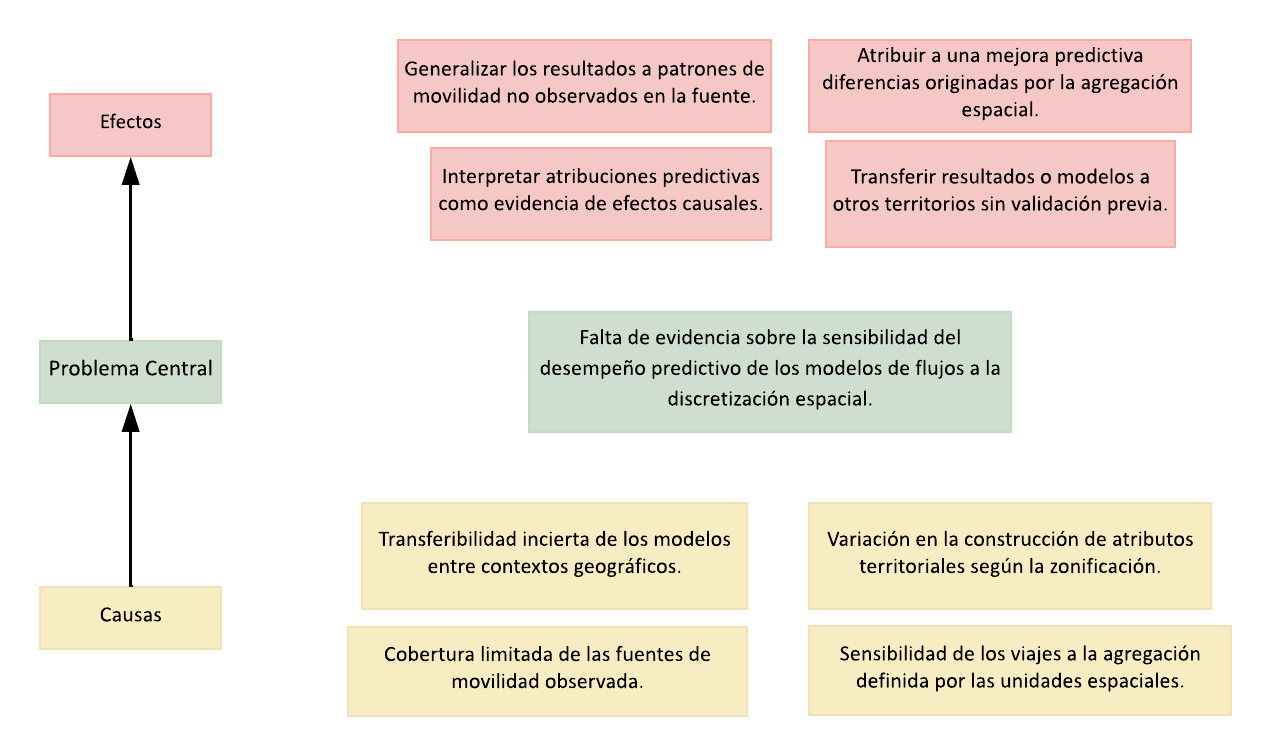
\includegraphics[width=\textwidth,keepaspectratio]{figures/arbol_del_problema.png}
	\caption{Árbol del problema: causas, problema central y efectos. Fuente: Elaboración propia.}
	\label{fig:arbol_problema}
\end{figure}

La Figura~\ref{fig:arbol_problema} sitúa como problema central la falta de evidencia sobre la sensibilidad del desempeño predictivo de los modelos de flujos a la discretización espacial. En esta memoria, dicha sensibilidad se examina para el transporte público de Santiago mediante la comparación entre Zona 777 y H3.

Las causas representadas son la cobertura limitada de las fuentes de movilidad observada, la sensibilidad de los viajes a la agregación definida por las unidades espaciales, la variación en la construcción de atributos territoriales según la zonificación y la transferibilidad incierta de los modelos entre contextos geográficos.

Como efectos, la falta de evidencia puede llevar a atribuir a una mejora predictiva diferencias originadas por la agregación espacial, generalizar resultados a patrones de movilidad no observados en la fuente, interpretar atribuciones predictivas como evidencia de efectos causales o transferir resultados o modelos a otros territorios sin validación previa. Estos efectos corresponden a riesgos metodológicos para la interpretación de resultados, no a efectos medidos sobre la inversión pública. Su posible utilidad para la planificación depende de la evidencia obtenida.

\subsection{Objetivo General}

Evaluar la sensibilidad de \textit{Deep Gravity} y de sus modelos de referencia frente a la discretización espacial Zona 777--H3, a partir de una cohorte DTPM común, trazable y reproducible para Santiago de Chile.

\subsection{Objetivos Específicos}
\label{sec:objetivos_especificos}

\begin{enumerate}
    \item Auditar y adaptar el código de referencia para verificar su funcionamiento y asegurar la trazabilidad de las ejecuciones.
    \item Reconstruir viajes canónicos desde las tablas DTPM de viajes y etapas, definir una cohorte común y delimitar el núcleo urbano de Santiago mediante reglas espaciales reproducibles.
    \item Construir representaciones comparables mediante Zona 777 y H3, evaluar la factibilidad de las resoluciones H3-r3 a H3-r8 y seleccionar candidatas para la evaluación experimental.
    \item Construir atributos de población y de OpenStreetMap con fuentes, unidades y procedimientos de agregación y normalización explícitos.
    \item Entrenar y evaluar \textit{Deep Gravity} frente a los modelos de referencia uniforme, de atracción de entrenamiento y de gravedad exponencial, mediante una medida de solapamiento de flujos observados y predichos, el componente común de viajeros (\textit{Common Part of Commuters}, CPC), sobre particiones espaciales comparables.
    \item Evaluar, como análisis complementario, la viabilidad de obtener atribuciones predictivas estables de las características territoriales mediante técnicas de inteligencia artificial explicable (XAI), documentando la configuración, los controles y el alcance efectivo del análisis.
\end{enumerate}

\newpage
\secnumbersection{MARCO CONCEPTUAL}

Este capítulo presenta los fundamentos de la modelación de flujos origen-destino. Describe los modelos clásicos como antecedentes teóricos y expone la formulación de \textit{Deep Gravity}, distinguiendo la publicación original de la adaptación utilizada en Santiago. Luego introduce los métodos de atribución de predicciones, las fuentes geoespaciales y el contexto de movilidad. El procedimiento experimental de esta memoria se especifica en el Capítulo~\ref{sec:cap4}.

% ----------------------------------------------------------------
\subsection{Movilidad urbana y flujos origen-destino}
% ----------------------------------------------------------------

La movilidad urbana comprende el conjunto de desplazamientos que realizan las personas entre distintas ubicaciones de la ciudad en un período de tiempo determinado \cite{liu2024interdisciplinary}. Comprender estos desplazamientos es un insumo fundamental para la planificación del transporte, el diseño de infraestructura vial y la formulación de políticas públicas basadas en evidencia.

Una representación sintética y cuantitativa de la movilidad urbana es la matriz origen-destino (matriz OD). Formalmente, dado un conjunto de $n$ zonas geográficas $\mathcal{Z} = \{z_1, z_2, \dots, z_n\}$ que particionan el área de estudio, el flujo $T_{ij}$ representa el número de viajes que se realizan desde la zona de origen $z_i$ hasta la zona de destino $z_j$ en un intervalo de tiempo fijo:
\begin{equation}
    \mathbf{T} \in \mathbb{R}^{n \times n}, \quad T_{ij} \geq 0 \quad \forall\, i, j \in \{1, \dots, n\}
    \label{eq:matriz_od}
\end{equation}
La colección de todos los flujos posibles entre pares de zonas conforma la matriz OD. Cada fila $i$ representa los flujos salientes desde una zona de origen, y cada columna $j$ los flujos entrantes hacia una zona de destino.

Obtener la matriz OD mediante observación directa, a través de encuestas domiciliarias, aforos de tráfico o registros de tarjetas de pago, es costoso y poco frecuente. Esta limitación ha motivado el desarrollo de modelos generativos de flujos, capaces de estimar $\mathbf{T}$ a partir de características observables del territorio, como la distribución de la población o la presencia de equipamientos urbanos, sin depender exclusivamente de mediciones directas \cite{simini2021deep}.

El problema de generación de flujos se formula de la siguiente manera: dado un conjunto de zonas $\mathcal{Z}$, sus características geoespaciales y los flujos totales salientes por zona $O_i = \sum_j T_{ij}$, estimar los flujos por par origen-destino $\hat{T}_{ij}$ para todos los pares $(i, j)$.

% ----------------------------------------------------------------
\subsection{Modelos clásicos de generación de flujos}
% ----------------------------------------------------------------

La estimación de flujos origen-destino cuenta con una tradición extensa en la geografía cuantitativa. Los modelos que se describen a continuación constituyen antecedentes teóricos de esta memoria. Los modelos de referencia utilizados en la evaluación de Santiago se especifican en el Capítulo~\ref{sec:cap4}.

\subsubsection{Modelo gravitatorio}

El modelo gravitatorio de movilidad establece una analogía con la ley de gravitación universal de Newton. La aplicación de este principio a los fenómenos sociales cuenta con antecedentes desde el siglo XIX. Posteriormente, Zipf \cite{zipf1946p} lo formalizó en 1946 para la predicción de flujos. Su formulación postula que el volumen de desplazamientos entre dos zonas es directamente proporcional al producto de sus masas (habitualmente la población) e inversamente proporcional a la distancia que las separa:
\begin{equation}
    T_{ij} = k \cdot \frac{P_i^{\,\alpha} \cdot P_j^{\,\beta}}{d_{ij}^{\,\gamma}}
    \label{eq:gravedad}
\end{equation}
donde $P_i$ y $P_j$ son las poblaciones de las zonas de origen y destino, $d_{ij}$ es la distancia entre sus centroides, $k$ es una constante de proporcionalidad, y $\alpha$, $\beta$, $\gamma$ son parámetros que deben calibrarse con datos observados. Zipf verificó empíricamente esta relación mediante datos de tráfico de buses, ferrocarriles y llamadas telefónicas entre ciudades de Estados Unidos. Los coeficientes obtenidos se aproximan a la unidad en todos los casos.

La formulación de la ecuación \eqref{eq:gravedad} recibe el nombre de \textit{modelo de gravedad no restringido}. En la práctica, para garantizar que los flujos generados sean consistentes con los totales salientes observados, se utiliza la versión \textit{restringida en origen} (\textit{singly-constrained}), que normaliza los flujos de cada origen sobre todos sus destinos posibles:
\begin{equation}
    \hat{T}_{ij} = O_i \cdot \frac{P_j^{\,\beta}\, f(d_{ij})}{\displaystyle\sum_{k} P_k^{\,\beta}\, f(d_{ik})}
    \label{eq:gravedad_restringida}
\end{equation}
donde $O_i = \sum_j T_{ij}$ es el flujo total saliente de la zona $i$ y $f(d_{ij})$ es una función de disuasión por distancia, que puede adoptar una forma exponencial, $f(d_{ij})=e^{-\lambda d_{ij}}$, con $\lambda>0$, o una ley de potencia, $f(d_{ij})=d_{ij}^{-\gamma}$, con $\gamma>0$ y $d_{ij}>0$\footnote{Existe también la versión \textit{doblemente restringida} (\textit{doubly-constrained}), que impone conservación tanto de los flujos salientes $O_i$ como de los flujos entrantes $D_j = \sum_i T_{ij}$. \textit{Deep Gravity} utiliza exclusivamente la versión restringida en origen.}.

Las limitaciones de un modelo gravitatorio dependen de su especificación \cite{liu2024interdisciplinary}. La versión presentada relaciona población, distancia y flujo mediante parámetros calibrados con observaciones. Los usos del suelo, los equipamientos y la infraestructura de transporte quedan fuera de su vector explicativo. Esta caracterización corresponde a esa formulación; otras extensiones de la familia gravitatoria incorporan atributos diferentes. Su adecuación y la transferencia de sus parámetros requieren evaluación empírica.

\subsubsection{Modelo de oportunidades intervinientes}

Stouffer \cite{stouffer1940intervening} propuso en 1940 una perspectiva alternativa al modelo gravitatorio, en la que la distancia funciona como un contenedor espacial de oportunidades. Su hipótesis central es que el número de personas que se desplazan a una zona de destino es directamente proporcional al número de oportunidades en ese destino e inversamente proporcional al número de oportunidades intervinientes entre el origen y el destino.

Formalmente, sea $y$ el número de personas que se desplazan desde un origen hasta una banda circular de anchura $\Delta s$, y sea $x$ el número acumulado de oportunidades entre el origen y la distancia $s$. Stouffer postula:
\begin{equation}
    \Delta y = a \cdot \frac{\Delta x}{x}
    \label{eq:stouffer}
\end{equation}
Integrando esta expresión diferencial, el número total de personas que se detienen dentro de un círculo de radio $s$ desde el origen es:
\begin{equation}
    y = a \cdot \ln f(s) + c
    \label{eq:stouffer_integral}
\end{equation}
donde $f(s)$ es el número acumulado de oportunidades dentro de ese radio y $c$ es una constante de integración. Stouffer verificó empíricamente esta formulación con datos de movilidad residencial en Cleveland, Ohio (1933-1935). Los resultados muestran una buena correspondencia entre los flujos observados y los predichos por el modelo.

Liu y Yan \cite{liu2020intervening} formalizaron y extendieron esta familia de modelos de manera rigurosa. Para describir su funcionamiento, es necesario precisar tres conceptos fundamentales:

\begin{itemize}
    \item \textbf{Oportunidades de un lugar} ($m_l$): cantidad de oportunidades que ofrece el lugar $l$ para satisfacer el propósito del desplazamiento. En la práctica se asume que $m_l$ es proporcional a la población del lugar.
    \item \textbf{Oportunidades intervinientes} ($s_{ij}$): suma de oportunidades de todos los lugares cuya distancia al origen $i$ es menor que $d_{ij}$, excluyendo el propio origen $i$ y el destino $j$. Si se incluyen origen y destino se utiliza la notación $S_{ij} = m_i + s_{ij} + m_j$.
    \item \textbf{Valor de beneficio de una oportunidad} ($z$): utilidad o recompensa que una oportunidad reporta al viajero. Se modela como variable aleatoria continua con distribución $p(z)$.
\end{itemize}

El modelo de Stouffer establece que cada individuo que parte del origen $i$ ordena todos los destinos potenciales por distancia creciente y se detiene en cada lugar con una probabilidad fija proporcional al parámetro $\alpha$. Bajo este mecanismo, la probabilidad de que un individuo en $i$ elija el destino $j$ adopta la forma \cite{stouffer1940intervening, liu2020intervening}:
\begin{equation}
    P_{ij} = \frac{e^{-\alpha(S_{ij} - m_j)} - e^{-\alpha S_{ij}}}{1 - e^{-\alpha M}}
    \label{eq:io_formal}
\end{equation}
donde $m_j$ es la cantidad de oportunidades del destino $j$, $S_{ij}$ es el total de oportunidades en el círculo de radio $d_{ij}$ centrado en $i$ (incluyendo origen y destino), $\alpha$ es el parámetro de absorción a calibrar con datos históricos, y $M = \sum_k m_k$ es el total de oportunidades del sistema. La ecuación \eqref{eq:io_formal} muestra que la probabilidad de elegir $j$ crece con las oportunidades del destino $m_j$ y decrece con el número de oportunidades intervinientes $s_{ij}$: cuanto mayor es la competencia en el camino, menor la probabilidad de alcanzar el destino.

La principal limitación del modelo original de Stouffer es que contiene el parámetro $\alpha$, que debe calibrarse mediante datos históricos de flujo observado. Esta dependencia paramétrica restringe su aplicabilidad cuando no se dispone de matrices OD previas, y motivó el desarrollo de modelos libres de parámetros basados en el mismo concepto de oportunidades intervinientes.

\subsubsection{Modelo de radiación}

Simini et al. \cite{simini2012universal} propusieron en 2012 el modelo de radiación como una alternativa libre de parámetros al modelo gravitatorio. El modelo establece una analogía con los procesos de radiación y absorción en física de partículas. Su mecanismo se basa en un proceso estocástico de toma de decisiones locales: cada individuo en un origen busca la mejor oportunidad disponible dentro de radios geográficos crecientes y se desplaza hacia el destino donde la encuentra.

El mecanismo es el siguiente. Se asigna a cada oportunidad un valor de beneficio $z$ extraído de una distribución de probabilidad $p(z)$. La probabilidad de que un individuo en la zona $i$ elija la zona $j$ como destino es la probabilidad de que el mejor beneficio dentro de $j$ supere al mejor beneficio disponible dentro del círculo de radio $d_{ij}$ centrado en $i$ (excluyendo $i$ y $j$). Esta probabilidad es:
\begin{equation}
    p(n_j \mid m_i, s_{ij}) = \frac{m_i \, n_j}{(m_i + s_{ij})(m_i + n_j + s_{ij})}
    \label{eq:radiacion}
\end{equation}
donde $m_i$ es la población de la zona de origen $i$, $n_j$ es la población de la zona de destino $j$, y $s_{ij}$ es la población total dentro de un círculo de radio $d_{ij}$ centrado en $i$, excluyendo las poblaciones de $i$ y de $j$. El flujo esperado entre $i$ y $j$ es entonces:
\begin{equation}
    \langle T_{ij} \rangle = T_i \cdot \frac{m_i \, n_j}{(m_i + s_{ij})(m_i + n_j + s_{ij})}
    \label{eq:radiacion_flujo}
\end{equation}
donde $T_i = \sum_j T_{ij}$ es el flujo total saliente de la zona $i$. Una propiedad destacable del modelo de radiación es que satisface automáticamente la restricción de conservación de flujos: $\sum_j \langle T_{ij} \rangle = T_i$, sin necesidad de calibración de parámetros adicionales.

Simini et al. \cite{simini2012universal} validaron el modelo sobre datos de \textit{commuting} del censo de Estados Unidos (2000). Los resultados muestran que el modelo de radiación supera al modelo gravitatorio en la reproducción de flujos observados, especialmente en viajes de corta distancia, que el modelo gravitatorio tiende a sobreestimar.

\paragraph{Variantes del modelo de radiación.} La solidez del modelo original motivó diversas extensiones para adaptar su mecanismo a diferentes contextos. Ren et al. \cite{ren2014predicting} propusieron una versión basada en tiempo de viaje en lugar de distancia euclidiana, incorporando así la resistencia real de la red de transporte. Kang et al. \cite{kang2015generalized} formularon un modelo de radiación generalizado que introduce parámetros de escala y restricciones explícitas de producción y atracción, mejorando la precisión en contextos con heterogeneidad espacial marcada. Yang et al. \cite{yang2014limits} extendieron el modelo para incorporar la distribución no homogénea de oportunidades en el espacio, relevante en regiones con alta segregación funcional del suelo.

\paragraph{Limitación del modelo de radiación a escala intraurbana.} A pesar de su éxito en la predicción de \textit{commuting} interurbano, el modelo de radiación presenta una limitación estructural cuando se aplica a la escala intraurbana \cite{yan2014population, liu2020intervening}. Su supuesto central, que cada individuo elige el destino más cercano cuyo beneficio supera al del origen, refleja adecuadamente el comportamiento en la búsqueda de empleo a larga distancia (donde la proximidad es costosa), pero no captura la lógica real de los desplazamientos dentro de una ciudad. En entornos urbanos, las personas consideran simultáneamente el conjunto de destinos disponibles en toda la ciudad, sin restringirse a los más cercanos. Estudios empíricos sobre datos de transporte público en diversas ciudades confirman que el modelo de radiación subestima sistemáticamente los flujos intraurbanos de largo alcance \cite{yan2014population}. Adicionalmente, el modelo utiliza exclusivamente la población como \textit{proxy}\footnote{Una variable \textit{proxy} es una medida indirecta que se emplea en sustitución de una variable inobservable, asumiendo que existe una fuerte correlación estadística entre ambas.} de oportunidades, sin incorporar características del tejido urbano como el uso de suelo o la distribución de actividades económicas. Estas limitaciones fueron el punto de partida para el desarrollo del modelo de oportunidades ponderadas por población, descrito en la Sección \ref{sec:modelos_evolucion}, y justifican el uso de modelos basados en aprendizaje profundo capaces de representar el tejido urbano más allá de la simple distribución poblacional, como \textit{Deep Gravity}.

% ----------------------------------------------------------------
\subsection{Aprendizaje profundo aplicado a la movilidad}
% ----------------------------------------------------------------

El aprendizaje profundo (\textit{deep learning}) es un subcampo del aprendizaje automático que utiliza redes neuronales con múltiples capas de transformaciones no lineales para aprender representaciones jerárquicas de los datos \cite{liu2024interdisciplinary}. Su aplicación a la predicción de flujos de movilidad ha permitido incorporar un conjunto amplio de variables geoespaciales y capturar relaciones no lineales que los modelos clásicos no pueden representar.

Una red neuronal \textit{feedforward} (de propagación hacia adelante) con $L$ capas ocultas transforma un vector de entrada $\mathbf{x} \in \mathbb{R}^d$ mediante una secuencia de transformaciones afines seguidas de funciones de activación no lineales:
\begin{equation}
    \mathbf{z}^{(0)} = \sigma\!\left(W^{(0)}\,\mathbf{x}\right), \qquad
    \mathbf{z}^{(\ell)} = \sigma\!\left(W^{(\ell)}\,\mathbf{z}^{(\ell-1)}\right), \quad \ell = 1, \dots, L-1
    \label{eq:feedforward}
\end{equation}
donde $W^{(\ell)}$ es la matriz de pesos de la capa $\ell$ y $\sigma(\cdot)$ es la función de activación, comúnmente ReLU ($\max(0, x)$) o su variante LeakyReLU ($\max(\alpha x, x)$ con $\alpha$ pequeño), que mitiga el problema del gradiente desvanecido en redes profundas.

En el contexto de la generación de flujos, el aprendizaje profundo ha sido aplicado de múltiples formas: como extensión no lineal del modelo gravitatorio \cite{simini2021deep}, mediante redes neuronales de grafos que modelan la estructura espacial de las zonas, y mediante modelos de series de tiempo que capturan la evolución temporal de los flujos \cite{luca2024tsmob}. Esta memoria se enfoca en el primero de estos enfoques, implementado a través del modelo \textit{Deep Gravity}.

% ----------------------------------------------------------------
\subsection{Deep Gravity}
% ----------------------------------------------------------------

\textit{Deep Gravity} es un modelo de generación de flujos de movilidad propuesto por Simini et al. \cite{simini2021deep} en 2021. Su contribución central es demostrar que el modelo gravitatorio clásico restringido en origen (ecuación \ref{eq:gravedad_restringida}) es formalmente equivalente a una red neuronal lineal de una sola capa con salida \textit{softmax}, y que reemplazar esa capa lineal por una red neuronal profunda permite capturar relaciones no lineales entre las características del territorio y los flujos observados.

\subsubsection{Formulación matemática}

El modelo gravitatorio restringido en origen puede reescribirse como un modelo lineal generalizado con distribución multinomial. Para un origen $i$, la probabilidad de que un viaje se dirija al destino $j$ es:
\begin{equation}
    p_{ij} = \frac{\exp\!\left(\boldsymbol{\beta}^{\top}\,\mathbf{x}(l_i, l_j)\right)}{\displaystyle\sum_{k} \exp\!\left(\boldsymbol{\beta}^{\top}\,\mathbf{x}(l_i, l_k)\right)}
    \label{eq:dg_glm}
\end{equation}
donde $\mathbf{x}(l_i, l_j) = \bigl[\ln P_j,\, d_{ij}\bigr]$ es el vector de características del par $(i, j)$, y $\boldsymbol{\beta} = [\beta_1, \beta_2]$ son los parámetros del modelo.

Con distancia sin transformar, el numerador es proporcional a $P_j^{\beta_1}e^{\beta_2 d_{ij}}$; la disuasión exponencial corresponde a $\beta_2<0$. Una ley de potencia se obtiene incorporando $\ln d_{ij}$ en lugar de $d_{ij}$, para distancias positivas. Ambas son formulaciones gravitatorias, con funciones de disuasión distintas.

La formulación publicada utiliza la siguiente entropía cruzada entre distribuciones de destino normalizadas por origen, para orígenes con $O_i>0$:
\begin{equation}
    H = -\sum_i \sum_j \frac{T_{ij}}{O_i} \ln p_{ij}
    \label{eq:dg_loss}
\end{equation}
Esta expresión asigna el mismo peso a cada origen. La pérdida efectiva de Santiago pondera las contribuciones por la masa observada, $-\sum_i\sum_j T_{ij}\ln p_{ij}$, como se especifica en la ecuación~\eqref{eq:perdida_multinomial_santiago}. Por tanto, las dos expresiones definen objetivos de entrenamiento distintos.
\textit{Deep Gravity} reemplaza el producto interno lineal $\boldsymbol{\beta}^{\top}\,\mathbf{x}(l_i, l_j)$ por una red neuronal profunda $f_\theta(\mathbf{x}(l_i, l_j))$ que produce un \textit{score} escalar. Las probabilidades de destino se obtienen mediante \textit{softmax} sobre los \textit{scores} de todos los destinos candidatos desde el origen $i$:
\begin{equation}
    p_{ij} = \frac{\exp\!\left(f_\theta\!\left(\mathbf{x}(l_i, l_j)\right)\right)}{\displaystyle\sum_{k} \exp\!\left(f_\theta\!\left(\mathbf{x}(l_i, l_k)\right)\right)}
    \label{eq:dg_softmax}
\end{equation}
El flujo estimado desde $i$ hacia $j$ es entonces $\hat{T}_{ij} = O_i \cdot p_{ij}$. El total $O_i$ se considera conocido; la tarea predictiva consiste en estimar la distribución de ese flujo entre destinos.

\subsubsection{Arquitectura de la red neuronal}

En la arquitectura descrita por Simini et al. \cite{simini2021deep}, la función $f_\theta$ se implementa como una red neuronal \textit{feedforward} de 15 capas ocultas con activación LeakyReLU. Las primeras 6 capas tienen dimensión 256 y las 9 restantes dimensión 128. La capa de salida produce un escalar:
\begin{align}
    \mathbf{z}^{(0)} &= \text{LeakyReLU}\!\left(W^{(0)}\,\mathbf{x}(l_i, l_j)\right) \nonumber \\
    \mathbf{z}^{(\ell)} &= \text{LeakyReLU}\!\left(W^{(\ell)}\,\mathbf{z}^{(\ell-1)}\right), \quad \ell = 1, \dots, 14 \nonumber \\
    f_\theta\!\left(\mathbf{x}(l_i, l_j)\right) &= \mathbf{w}^{\top}\,\mathbf{z}^{(14)}
    \label{eq:dg_red}
\end{align}
Esta distribución de anchos corresponde a la arquitectura descrita en la publicación. La implementación utilizada en Santiago tiene cinco capas ocultas de 256 unidades y diez de 128; su configuración efectiva se documenta en la Sección~\ref{sec:configuracion_entrenamiento}.
El protocolo publicado emplea RMSprop, con momento 0,9, tasa de aprendizaje $5\times10^{-6}$, lotes de 64 orígenes y hasta 512 destinos muestreados por origen. El muestreo calcula la normalización sobre un subconjunto de candidatos durante el entrenamiento. La configuración de Santiago, documentada en la Sección~\ref{sec:configuracion_entrenamiento}, usa lotes de ocho orígenes y el soporte completo de destinos para entrenar y evaluar. Los parámetros de los experimentos finales se fijan en su diseño específico.

\subsubsection{Vector de características geoespaciales}

En la formulación de referencia \cite{simini2021deep}, el vector de entrada reúne atributos del origen y del destino, población y distancia. Su estructura puede representarse mediante el siguiente esquema de 39 componentes:
\begin{equation}
    \mathbf{x}(l_i, l_j) = \bigl[\mathbf{f}(l_i),\; \mathbf{f}(l_j),\; \ln P_i,\; \ln P_j,\; d_{ij}\bigr]
    \label{eq:dg_features}
\end{equation}
donde $\mathbf{f}(l)\in\mathbb{R}^{18}$ reúne atributos geoespaciales de la ubicación $l$, $P_i$ y $P_j$ representan la población asociada a ambos extremos y $d_{ij}$ es la distancia entre sus representantes espaciales. La procedencia de las variables y sus transformaciones deben identificarse en cada aplicación.

En Santiago se utiliza un conjunto de 19 atributos por ubicación y 39 componentes por par. Incluye densidad de población censal, coberturas de suelo, densidades viales y atributos de equipamientos y servicios. Su construcción, orden y transformación se definen en la Sección~\ref{sec:features_osm}. El vector conserva 39 componentes por par, pero su contenido corresponde a fuentes y transformaciones distintas. La población de Santiago procede del Censo 2024 y se expresa como densidad después de la interpolación areal; su especificación difiere de las que usan logaritmos de población total o flujo saliente observado.

La agregación espacial depende de la magnitud del atributo. En Santiago, la densidad de población se expresa en personas por km$^2$, la densidad de puntos de interés en puntos por km$^2$ y la densidad vial en km de vías por km$^2$. La cobertura corresponde al área de la unión de polígonos de una categoría dividida por el área de la unidad, por lo que es una proporción adimensional entre cero y uno. Estas operaciones se distinguen de las transformaciones y la estandarización previas al entrenamiento, descritas en la Sección~\ref{sec:features_osm}.

\subsubsection{Resultados y desempeño}

Simini et al. \cite{simini2021deep} evaluaron \textit{Deep Gravity} sobre flujos censales de \textit{commuting} en Inglaterra e Italia y flujos derivados de telefonía móvil en el estado de Nueva York, utilizando la métrica \textit{Common Part of Commuters} (CPC), definida como:
\begin{equation}
    \text{CPC}(\hat{\mathbf{T}}, \mathbf{T}) = \frac{2\,\displaystyle\sum_{i,j} \min\!\left(\hat{T}_{ij},\, T_{ij}\right)}{\displaystyle\sum_{i,j} \hat{T}_{ij} + \displaystyle\sum_{i,j} T_{ij}}
    \label{eq:cpc}
\end{equation}
Cuando la masa del denominador es positiva, la métrica CPC toma valores en $[0,1]$, donde 1 indica coincidencia exacta entre flujos generados y reales. Es equivalente al índice de Sørensen-Dice aplicado a flujos. En los experimentos publicados, \textit{Deep Gravity} supera al modelo gravitatorio clásico en todos los contextos evaluados. Las mejoras en CPC global alcanzan hasta un 190\% en Inglaterra y un 1.066\% en el estado de Nueva York. El estudio también evaluó la transferencia geográfica. Entrenado en algunas ciudades del Reino Unido, mantuvo un desempeño similar al evaluarse en ciudades no vistas durante el entrenamiento. En el caso de Nueva York, la publicación aproxima la población mediante flujo saliente observado; Santiago utiliza otra definición de atributos. La auditoría técnica verifica la compatibilidad de la implementación y la evaluación de Santiago examina su desempeño empírico bajo el protocolo de esta memoria.

\subsubsection{Síntesis comparativa de modelos}

La Tabla~\ref{tab:comparacion_modelos} sintetiza antecedentes bibliográficos. La calibración, los atributos y el comportamiento intraurbano dependen de la variante; la evidencia latinoamericana se limita a las fuentes revisadas.

\begin{table}[H]
\centering
\caption{Comparación bibliográfica de modelos de flujos. Fuente: elaboración propia a partir de las referencias indicadas.}
\label{tab:comparacion_modelos}
\footnotesize
\renewcommand{\arraystretch}{1.15}
\begin{tabularx}{\textwidth}{@{}p{2.4cm}XXXXX@{}}
\toprule
\textbf{Modelo} &
\textbf{Atributos considerados} &
\textbf{Calibración} &
\textbf{Escala intraurbana} &
\textbf{Interpretación de la predicción} &
\textbf{Evidencia latinoamericana} \\
\midrule
Gravitatorio clásico \cite{zipf1946p,liu2024interdisciplinary}
    & Población y distancia
    & Exponentes y disuasión
    & Evaluación según contexto
    & Formulación explícita
    & --- \\
Oportunidades intervinientes \cite{stouffer1940intervening,liu2020intervening}
    & Oportunidades y su distribución
    & Parámetro de absorción
    & Depende de la formulación
    & Formulación explícita
    & --- \\
Radiación original \cite{simini2012universal,yan2014population}
    & Población como aproximación de oportunidades
    & Sin parámetros de forma
    & Limitaciones documentadas
    & Formulación explícita
    & --- \\
Variantes de oportunidades intervinientes \cite{yan2014population,liu2019opportunity}
    & Oportunidades, habitualmente aproximadas por población
    & Depende de la variante
    & Evaluadas en los contextos citados
    & Formulación explícita
    & --- \\
\textit{Deep Gravity} \cite{simini2021deep}
    & Población, atributos territoriales y distancia
    & Pesos de la red
    & Evaluación según contexto
    & Atribución posterior, como SHAP
    & --- \\
\bottomrule
\end{tabularx}

\smallskip
\begin{minipage}{\textwidth}
\footnotesize
Las celdas con --- registran la ausencia de aplicaciones latinoamericanas en el corpus bibliográfico revisado. Las formulaciones explícitas permiten inspeccionar supuestos; las explicaciones causales exigen un diseño de evaluación específico. SHAP reúne aproximaciones agnósticas aplicables a modelos diversos, incluidas redes profundas \cite{lundberg2017shap}. El artículo original de \textit{Deep Gravity} ya incorpora un análisis SHAP; esta memoria evaluó complementariamente la viabilidad de trasladar atribuciones a Santiago.
\end{minipage}
\end{table}

Estas características justifican la evaluación de \textit{Deep Gravity} en Santiago. Los capítulos siguientes establecen su desempeño bajo el diseño experimental de esta memoria y evalúan la viabilidad de las atribuciones.

% ----------------------------------------------------------------
\subsection{Explicabilidad en modelos de inteligencia artificial (XAI)}
% ----------------------------------------------------------------

La explicabilidad de la inteligencia artificial (\textit{eXplainable Artificial Intelligence}, XAI) se refiere al conjunto de técnicas que permiten comprender e interpretar las predicciones de modelos de aprendizaje automático complejos \cite{lundberg2017shap}. En el contexto de la planificación del transporte, la explicabilidad es relevante no solo desde el punto de vista académico, para estudiar cómo las variables de entrada contribuyen a las predicciones, sino también desde el punto de vista institucional, ya que permite a los planificadores auditar las predicciones del modelo.

\subsubsection{Valores SHAP}

SHAP (\textit{SHapley Additive exPlanations}), propuesto por Lundberg y Lee \cite{lundberg2017shap}, es un método de explicabilidad que fundamenta la importancia de cada variable en la teoría de juegos cooperativos de Shapley. La contribución de la característica $i$ a la predicción del modelo para una instancia $\mathbf{x}$ se define como:
\begin{equation}
    \phi_i(f, \mathbf{x}) = \sum_{S \subseteq \mathcal{F} \setminus \{i\}} \frac{|S|!\,(|\mathcal{F}|-|S|-1)!}{|\mathcal{F}|!}\,\bigl[f(S \cup \{i\}) - f(S)\bigr]
    \label{eq:shap}
\end{equation}
donde $\mathcal{F}$ es el conjunto de todas las características, $S$ es una coalición de características que no incluye a $i$, y $f(S)$ es la predicción del modelo usando solo las características en $S$. El valor $\phi_i$ representa la contribución marginal promedio de la característica $i$ sobre todas las posibles coaliciones de características.

Los valores SHAP satisfacen tres propiedades deseables: \textit{eficiencia} (la suma de todos los valores SHAP es igual a la diferencia entre la predicción y el valor base), \textit{simetría} (características con igual contribución marginal reciben igual valor SHAP) y \textit{dummy} (características sin influencia reciben valor cero). En conjunto, estas propiedades garantizan una atribución justa y consistente de importancias.

Los valores SHAP permiten estudiar la contribución de los atributos a una predicción con respecto a una referencia. En esta memoria, el análisis complementario incluyó aproximaciones de Shapley con referencias de entrenamiento y controles de estabilidad predefinidos. Los controles situaron este componente en una evaluación metodológica del procedimiento. Las atribuciones describen propiedades de las predicciones.

\subsubsection{Gradientes integrados}

Los \textit{Integrated Gradients} \cite{sundararajan2017axiomatic} son un método de atribución basado en el gradiente de la función del modelo con respecto a las variables de entrada. A diferencia de SHAP, que se fundamenta en la teoría de juegos cooperativos, los \textit{Integrated Gradients} derivan las atribuciones directamente de la estructura diferencial de la red neuronal. Para una predicción $f(\mathbf{x})$ y una entrada de referencia $\mathbf{x}'$, la atribución de la característica $i$ se define como:
\begin{equation}
    \text{IG}_i(\mathbf{x}) = (x_i - x_i') \cdot \int_0^1 \frac{\partial f\!\left(\mathbf{x}' + \alpha(\mathbf{x} - \mathbf{x}')\right)}{\partial x_i}\,\mathrm{d}\alpha
    \label{eq:ig}
\end{equation}
El método satisface dos propiedades axiomáticas que lo distinguen de otras técnicas de atribución: \textit{sensibilidad} (si la entrada y la referencia difieren en una sola característica y producen predicciones distintas, esa característica recibe atribución no nula) e \textit{invariancia a la implementación} (la atribución depende únicamente de la función matemática que computa la red, no de su arquitectura interna). Estas propiedades lo hacen complementario a SHAP, que satisface eficiencia, simetría y dummy.

La elección de la entrada de referencia $\mathbf{x}'$ es un aspecto crítico del método. El vector nulo ($\mathbf{x}' = \mathbf{0}$) es una convención habitual en clasificación de imágenes, pero su significado depende de las variables y de su preprocesamiento. Una densidad cartografiada puede ser cero; después de estandarizar, el valor cero representa la media de entrenamiento. La referencia debe definirse en el espacio de entrada del modelo y su elección requiere un análisis de sensibilidad. En Santiago, las referencias ensayadas se construyeron con orígenes de entrenamiento de cada rama para conservar la coherencia con las transformaciones del modelo.

Los gradientes integrados pueden considerarse una técnica complementaria para atribuir una salida diferenciable del modelo a sus entradas. En Santiago, la consulta crítica cubrió solo parte de la cobertura requerida aun al aumentar la cuadratura. Por ello, el método quedó en etapa de evaluación metodológica.

% ----------------------------------------------------------------
\subsection{OpenStreetMap como fuente de datos geoespaciales}
% ----------------------------------------------------------------

OpenStreetMap (OSM) es una base de datos geoespacial colaborativa y de libre acceso, construida y mantenida por una comunidad global de voluntarios desde su creación en 2004 \cite{haklay2008openstreetmap}. Su modelo de datos se articula en tres tipos de objetos geométricos: \textit{nodos} (puntos), \textit{vías} (secuencias de nodos que representan líneas o polígonos) y \textit{relaciones} (agrupaciones de nodos y vías con un significado semántico compartido). Cada objeto puede llevar asociados pares clave-valor denominados \textit{etiquetas} (\textit{tags}), que codifican su naturaleza (por ejemplo, \texttt{amenity=hospital} o \texttt{landuse=residential}).

Para modelar flujos de movilidad, OpenStreetMap aporta atributos de uso del suelo, vialidad, equipamientos y servicios. En esta memoria, el término \textit{amenities} se refiere a equipamientos y servicios urbanos; los atributos de OSM abarcan también información que no pertenece a ese conjunto. Los puntos de interés son una representación de algunas de estas entidades, mientras que otras se describen mediante áreas o líneas. La selección y construcción de los atributos empleados en Santiago se describe en la Sección~\ref{sec:features_osm}.

Una limitación reconocida de OSM es la heterogeneidad espacial de su cobertura. Estudios previos \cite{BarringtonLeigh2017} documentan variaciones de densidad y completitud asociadas, entre otros factores, al nivel socioeconómico y la accesibilidad; el patrón de Santiago se mide en esta memoria. El diagnóstico mide la presencia espacial de los atributos OSM que entraron a la red, tanto mediante su densidad como mediante la proporción de variables con valor positivo por unidad (Sección~\ref{sec:cobertura_atributos_osm}). Un valor cero registra ausencia cartografiada bajo las reglas de construcción. Estimar completitud externa o disponibilidad física de servicios requiere una fuente independiente de contraste.

% ----------------------------------------------------------------
\subsection{Contexto de la movilidad en Santiago de Chile}
% ----------------------------------------------------------------

El sistema integrado de transporte público de Santiago reúne buses, Metro y el servicio ferroviario Nos-Estación Central \cite{dtpm_informe_2024}. El área de estudio es un núcleo urbano referencial de 34 comunas y se diferencia de la cobertura operativa y de las delimitaciones estadísticas de la ciudad. La delimitación utilizada se describe en la Sección~\ref{sec:delimitacion}.

Las limitaciones de las fuentes de datos de movilidad disponibles para Santiago (la EOD de SECTRA y los registros de validación de la tarjeta bip!) se detallan en la Sección~\ref{sec:fuentes_movilidad}.

Esta memoria utiliza la entrega DTPM disponible entre el 1 y el 29 de noviembre de 2024. La unidad de análisis se reconstruye al unir viajes y etapas: las zonas y el factor de expansión principal provienen de viajes, mientras que las coordenadas UTM de subida y bajada se obtienen de etapas. La fuente permite construir matrices OD diarias y por período horario; el archivo del día 30 presentó errores de origen. Esta entrega constituye la principal fuente de flujos observados para el entrenamiento y la evaluación de \textit{Deep Gravity} en Santiago.

\newpage
\secnumbersection{TRABAJO RELACIONADO}

Este capítulo contrasta los supuestos, las necesidades de datos y las limitaciones de los enfoques de predicción de flujos origen-destino (OD) revisados en la literatura. El análisis fundamenta la elección de \textit{Deep Gravity} como arquitectura para evaluar el desempeño predictivo con atributos geoespaciales y su sensibilidad a la discretización en Santiago.

% ----------------------------------------------------------------
\subsection{Descubrimiento de patrones en la movilidad individual}
\label{sec:patrones_movilidad}
% ----------------------------------------------------------------

Durante mucho tiempo, la falta de datos de trayectoria masivos obligó a los investigadores a extrapolar los patrones de movilidad humana a partir de la dispersión de billetes de banco \cite{brockmann2006scaling}, asumiendo que los desplazamientos individuales seguían trayectorias puramente aleatorias y no acotadas, similares a los vuelos de Lévy (\textit{Lévy flights}). 

Este paradigma fue refutado por Gonz\'alez et al. \cite{gonzalez2008understanding}, quienes utilizaron registros masivos de telefonía móvil (CDR, por sus siglas en inglés) de 100.000 usuarios durante seis meses para analizar la movilidad humana a nivel microscópico. Su trabajo demostró que, a diferencia del movimiento browniano o de los vuelos de Lévy, las trayectorias humanas son altamente predecibles, regulares y están fuertemente confinadas espacialmente. Los autores introdujeron el concepto de \textit{radio de giro} para cuantificar la distancia típica recorrida por un individuo. Su análisis demostró que la aparente distribución pesada de saltos poblacionales es, en realidad, el resultado de agregar trayectorias individuales acotadas con una gran heterogeneidad en los radios de giro.

Esta contribución fue clave porque estableció que la movilidad urbana no es un fenómeno caótico, sino un sistema gobernado por rutinas (hogar-trabajo) y patrones espaciales predecibles. Esta previsibilidad estadística es la premisa fundamental que justifica el desarrollo de modelos matemáticos y algorítmicos para la predicción de flujos agregados.

% ----------------------------------------------------------------
\subsection{Unificación de modelos clásicos y enfoques continuos}
\label{sec:modelos_clasicos_continuos}
% ----------------------------------------------------------------

Con la confirmación de la regularidad en la movilidad humana, los esfuerzos se centraron en predecir los volúmenes de viaje entre distintas zonas de una ciudad o país. Tradicionalmente, este problema se abordó mediante el modelo gravitatorio \cite{zipf1946p} y el modelo de oportunidades intervinientes \cite{stouffer1940intervening}. Más tarde, el modelo de radiación \cite{simini2012universal} ofreció una solución libre de parámetros que superaba varias limitaciones empíricas de la formulación gravitatoria.

Estos modelos presentaban un problema matemático estructural: dependían fuertemente de la partición espacial utilizada (comunas, distritos, censos), lo que generaba inconsistencias espaciales. Además, salvo casos triviales, las formulaciones discretas como el modelo gravitatorio violaban la propiedad de \textit{aditividad}: el flujo hacia una región compuesta difería de la suma de los flujos hacia sus subregiones.

Para resolver esto, Simini, Maritan y N\'eda \cite{simini2013human} propusieron un marco unificado en el continuo. Los autores formularon un principio estocástico general de selección de beneficios laborales que preserva estrictamente la aditividad de los flujos. Además, demostraron que la gravedad, las oportunidades intervinientes y la radiación son, matemáticamente, casos particulares de una misma familia de procesos de selección espacial continua. Asimismo, introdujeron un parámetro de selección ($\lambda$) que flexibilizó el modelo de radiación para adaptarlo a diferentes escalas geográficas.

A pesar de su solidez teórica y elegancia matemática, este paradigma continuo arrastra una limitación fundamental de representación: asume que la cantidad de oportunidades en una región es estrictamente proporcional a su masa poblacional. En la realidad urbana, existe una profunda segregación funcional del suelo (zonas industriales, distritos financieros, áreas puramente residenciales) que rompe esta proporcionalidad lineal, exigiendo modelos capaces de entender el tejido urbano más allá de la simple aglomeración de personas.

% ----------------------------------------------------------------
\subsection{Evolución de los modelos de oportunidades intervinientes}
\label{sec:modelos_evolucion}
% ----------------------------------------------------------------

El concepto de oportunidades intervinientes de Stouffer \cite{stouffer1940intervening} inspiró, a lo largo de las décadas siguientes, una familia de modelos cada vez más sofisticados que buscaron superar las limitaciones paramétricas y escalares del modelo original. Liu y Yan \cite{liu2020intervening} ofrecen una revisión sistemática de esta evolución, identificando una línea de progresión que va desde el modelo de radiación hasta un marco unificado de comportamiento de destino. Esta sección sigue esa trayectoria, enfatizando los modelos más relevantes para el contexto intraurbano de la presente memoria.

\subsubsection{Modelo de oportunidades ponderadas por población}

Yan et al. \cite{yan2014population} identificaron en sus experimentos que el modelo de radiación falla sistemáticamente al predecir flujos dentro de una ciudad: sobreestima los flujos de corto alcance y subestima los de largo alcance intraurbano. Los autores argumentaron que el supuesto de selección secuencial por proximidad no refleja la realidad del viajero urbano, quien considera simultáneamente el conjunto completo de destinos disponibles en la ciudad.

Para corregir esto, Yan et al. \cite{yan2014population} propusieron el \textit{Modelo de Oportunidades Ponderadas por Población} (Population-Weighted Opportunity, PWO), en el que la probabilidad de elegir el destino $j$ desde el origen $i$ es proporcional a las oportunidades del destino e inversamente proporcional a las oportunidades totales dentro de un círculo centrado en el \emph{destino} $j$ con radio $d_{ij}$:
\begin{equation}
    P_{ij} = \frac{m_j}{S_{ji}}
    \label{eq:pwo}
\end{equation}
donde $m_j$ es la cantidad de oportunidades (población) del destino $j$, y $S_{ji} = m_j + s_{ji} + m_i$ es el total de oportunidades dentro del círculo de radio $d_{ij}$ centrado en $j$, incluyendo origen y destino. El cambio conceptual respecto al modelo de radiación es fundamental: en lugar de evaluar la competencia desde el origen, el modelo PWO evalúa la competencia desde el destino, capturando la lógica de atracción de un lugar sobre su entorno geográfico inmediato.

Al igual que el modelo de radiación, el modelo PWO es libre de parámetros: requiere únicamente la distribución de población de las zonas para generar predicciones, sin necesidad de calibración con datos históricos. Validado sobre datos de transporte público en múltiples ciudades chinas, el modelo PWO supera consistentemente al modelo de radiación en la predicción de viajes intraurbanos \cite{yan2014population}. Yan et al. \cite{yan2017unified} extendieron posteriormente este modelo combinándolo con un proceso de caminata aleatoria con memoria, logrando reproducir simultáneamente los patrones de movilidad a nivel individual y los flujos agregados a nivel poblacional.

\subsubsection{Modelos exploratorios: más allá de la selección secuencial}

Tanto el modelo de radiación como el modelo PWO comparten un supuesto implícito sobre el comportamiento del viajero. Según la terminología introducida retrospectivamente por Liu y Yan \cite{liu2020intervening} para clasificar los mecanismos de selección de destino, el modelo de radiación asume una \textit{tendencia cautelosa}: el individuo elige el destino más cercano que supera el beneficio del origen. El modelo PWO también incorpora una lógica de competencia local. En ambos casos, la distancia juega un papel restrictivo en la selección.

Investigaciones posteriores identificaron una tendencia exploratoria. En el ámbito de los procesos de evaluación y selección social, Sim et al. \cite{sim2015deliberate} describieron que, ante un beneficio suficientemente alto, los individuos consideran destinos más distantes. Liu y Yan \cite{liu2019opportunity} trasladaron formalmente este concepto al dominio de la movilidad espacial y propusieron el \textit{Modelo de Selección Prioritaria de Oportunidades} (Opportunity Priority Selection), en el que un individuo en $i$ elige el destino $j$ si su beneficio supera tanto al del origen como al de todas las oportunidades intervinientes:
\begin{equation}
    P_{ij} = \frac{m_j}{S_{ij}} = \frac{m_j}{m_i + s_{ij} + m_j}
    \label{eq:ops}
\end{equation}
donde $S_{ij} = m_i + s_{ij} + m_j$ es el total de oportunidades en el círculo de radio $d_{ij}$ centrado en el \emph{origen} $i$. Este modelo, al igual que el PWO, es libre de parámetros y fue validado con buenos resultados tanto para viajes intraurbanos como interurbanos.

\subsubsection{Modelo Unificado de Oportunidades}

La existencia de modelos con supuestos comportamentales tan distintos, el cauteloso modelo de radiación y el exploratorio modelo de selección prioritaria, planteó una pregunta natural: ¿qué modelo aplicar en cada contexto? Liu y Yan \cite{liu2020intervening} respondieron esta pregunta proponiendo el \textit{Modelo Unificado de Oportunidades} (Universal Opportunity Model), un marco general con dos parámetros que engloba a los modelos anteriores como casos especiales. La probabilidad de que un individuo en $i$ elija el destino $j$ se formula como:
\begin{equation}
    P_{ij} = \frac{(m_i + \alpha\, s_{ij})\, m_j}{\bigl[m_i + (\alpha + \beta)\, s_{ij}\bigr]\bigl[m_i + (\alpha + \beta)\, s_{ij} + m_j\bigr]}
    \label{eq:uom}
\end{equation}
donde $\alpha \geq 0$ es el parámetro de \textit{tendencia exploratoria} (cuán dispuesto está el individuo a alejarse buscando mayor beneficio) y $\beta \geq 0$ es el parámetro de \textit{tendencia cautelosa} (preferencia por destinos cercanos), sujetos a $\alpha + \beta \leq 1$. Los modelos previos emergen como casos particulares de esta formulación:

\begin{itemize}
    \item Si $\alpha = 0$, $\beta = 1$: la ecuación \eqref{eq:uom} se reduce a la ecuación \eqref{eq:radiacion} del modelo de radiación (comportamiento puramente cauteloso).
    \item Si $\alpha = 1$, $\beta = 0$: la ecuación \eqref{eq:uom} se reduce a la ecuación \eqref{eq:ops} del modelo de selección prioritaria (comportamiento puramente exploratorio).
\end{itemize}

Liu y Yan \cite{liu2020intervening} validaron el modelo sobre 14 conjuntos de datos de movilidad a distintas escalas: carga de mercancías, \textit{commuting} interurbano (EE.UU., Italia, Hungría), búsqueda de empleo, migración, viajes entre ciudades y viajes intraurbanos (Berlín, Londres, Beijing, Shenzhen, Suzhou). Sus resultados revelan un patrón sistemático: los flujos de \textit{commuting} y carga exhiben alta tendencia cautelosa (los individuos priorizan destinos cercanos de alto beneficio), mientras que los desplazamientos intraurbanos presentan valores bajos de ambos parámetros, indicando que la masa poblacional por sí sola es insuficiente para capturar la complejidad de la elección de destino en la ciudad. Este hallazgo es particularmente relevante para la presente memoria: sugiere que las variables de oportunidad basadas en población deben complementarse con atributos del tejido urbano para modelar adecuadamente los flujos en Santiago de Chile.

\paragraph{Aplicaciones colaterales.} Más allá de la movilidad de transporte, esta familia de modelos ha demostrado versatilidad en otros dominios. En el campo de la epidemiología, modelos como el de radiación y el PWO han sido utilizados para estimar probabilidades de contacto entre poblaciones y parametrizar la difusión espacial de enfermedades infecciosas, incluyendo estudios sobre la propagación de COVID-19 \cite{liu2020intervening}. Esta amplitud de aplicación evidencia la robustez conceptual del marco de oportunidades intervinientes.

% ----------------------------------------------------------------
\subsection{Deep Learning y modelos espacio-temporales en movilidad}
\label{sec:deep_learning_movilidad}
% ----------------------------------------------------------------

Para superar las limitaciones lineales y la dependencia exclusiva de la densidad poblacional, la literatura reciente ha migrado hacia el aprendizaje automático (\textit{Machine Learning}) y el aprendizaje profundo (\textit{Deep Learning}) \cite{liu2024interdisciplinary}. Las arquitecturas neuronales han demostrado una capacidad superior para capturar la no linealidad del entorno urbano.

Un avance significativo en esta línea es la incorporación explícita de Puntos de Interés (POIs) y características del entorno construido como variables condicionantes. Por ejemplo, Luca et al. \cite{luca2024tsmob} propusieron el \textit{framework} TS-Mob, que combina modelos fundacionales de series de tiempo (\textit{TimesFM}) con un módulo de atractividad gravitacional basado en perceptrones multicapa (MLP). Este modelo integra 16 categorías de POIs extraídas de bases de datos abiertas. Ello permite modular la probabilidad de atracción estructural de un destino en función de la oferta de servicios comerciales, educativos o de salud y de la población. Es importante distinguir este enfoque del de \textit{Deep Gravity}: mientras TS-Mob integra estas categorías en un módulo de atractividad temporal, la adaptación de \textit{Deep Gravity} de esta memoria utiliza un vector estático de atributos territoriales y distancia. Su composición y preprocesamiento se describen en la Sección~\ref{sec:features_osm}.

La transición hacia arquitecturas profundas introdujo requisitos de datos para controlar sobreajuste y dificultades de interpretación asociadas a sus arquitecturas de caja negra \cite{liu2024interdisciplinary}. Los estudios citados reportan menores errores y mayor CPC que los modelos clásicos; explicar una predicción individual sigue siendo una condición relevante para la adopción institucional.

% ----------------------------------------------------------------
\subsection{Generación de flujos mediante datos no convencionales}
\label{sec:flujos_no_convencionales}
% ----------------------------------------------------------------

En el estado del arte más reciente (2024-2025), la investigación ha explorado métodos para mitigar la dependencia de datos socioeconómicos hiperlocales o de costosas encuestas de transporte. Destaca el paradigma de inferencia mediante imágenes satelitales y modelos generativos de grafos.

Un estudio fundacional en esta línea metodológica es el de Xu et al. \cite{xu2025predicting}, quienes desarrollaron \textit{Imagery2Flow}, un modelo que emplea aprendizaje contrastivo y Redes de Atención en Grafos (GAT) para predecir flujos a partir de imágenes satelitales. Su investigación utiliza a \textit{Deep Gravity} como arquitectura de referencia en la literatura. Los autores demuestran que la versión con atributos espaciales (\textit{Deep Gravity-V}) supera con claridad a la versión puramente poblacional (\textit{Deep Gravity-P}). Este resultado respalda la utilidad predictiva de esos atributos en las condiciones evaluadas por los autores.

Posteriormente, Rong et al. \cite{rong2026satellites} extendieron este paradigma de inferencia satelital mediante \textit{GlODGen}, un generador global de flujos OD basado en modelos de difusión (\textit{Denoising Diffusion Networks}). Este \textit{framework} utiliza un codificador visual multimodal (\textit{RemoteCLIP}) para extraer un \textit{embedding} semántico de 1.024 dimensiones directamente desde imágenes satelitales de alta resolución. Los autores reportan que el aspecto visual del entorno urbano y un mapa global de población poseen una expresividad superior al 98\% respecto al uso de datos multisectoriales complejos (catastros, POIs, atributos socioeconómicos). Su modelo, entrenado en Estados Unidos, demostró transferibilidad a ciudades de Europa, China, Brasil y África.

Estos modelos presentan barreras prácticas para su aplicación. Pueden conservar sesgos geográficos de los contextos donde fueron entrenados y su desempeño es, además, sensible a la calidad de las imágenes satelitales. La representación del territorio mediante \textit{embeddings} puede dificultar la asociación directa entre los componentes aprendidos y categorías urbanas explícitas. Relacionar una predicción con equipamientos concretos requiere procedimientos de interpretación adicionales y validación; esa dificultad depende de la arquitectura, los datos y el método de explicación utilizado. El estudio de intervenciones urbanas con estas representaciones requiere una validación diseñada para vincular predicciones y efectos de intervención.

En el contexto latinoamericano, los antecedentes de aplicación de modelos computacionales para la generación de flujos son escasos. Spadon et al. \cite{spadon2019reconstructing} reconstruyeron redes de \textit{commuting} en la región metropolitana de São Paulo utilizando \textit{random forests} e indicadores urbanos municipales, demostrando la viabilidad de enfoques basados en aprendizaje automático para ciudades de la región. Su trabajo emplea arquitecturas de baja complejidad e indicadores urbanos municipales. Esta memoria evalúa empíricamente la adaptación de \textit{Deep Gravity} al transporte público de Santiago con atributos OSM y controles de explicabilidad.

% ----------------------------------------------------------------
\subsection{En Resumen}
% ----------------------------------------------------------------

La revisión permite comparar los supuestos, las necesidades de datos y las posibilidades de interpretación de los modelos:

\begin{itemize}
    \item Los modelos físicos y estadísticos clásicos (Secciones~\ref{sec:patrones_movilidad} y \ref{sec:modelos_clasicos_continuos}) ofrecen formulaciones explícitas; algunos marcos continuos incorporan propiedades de aditividad \cite{simini2013human}. Las versiones basadas en población y distancia restringen de antemano la relación entre esas variables y el flujo, mientras que otras formulaciones amplían sus atributos y supuestos.
    \item Los modelos de oportunidades intervinientes (Sección~\ref{sec:modelos_evolucion}) han dado lugar a formulaciones con distintos supuestos de selección de destino y requisitos de calibración. En las variantes revisadas, la población suele utilizarse como aproximación de las oportunidades, lo que limita la descripción de actividades urbanas específicas.
    \item Los modelos basados en aprendizaje profundo, series de tiempo e imágenes satelitales (Secciones~\ref{sec:deep_learning_movilidad} y \ref{sec:flujos_no_convencionales}) han mostrado capacidad predictiva en los contextos y protocolos evaluados por los estudios citados. Sus necesidades de cómputo y la interpretación de sus salidas dependen de la arquitectura, de los atributos y del método de explicación.
\end{itemize}

En este contexto metodológico, el uso del modelo \textit{Deep Gravity} \cite{simini2021deep}, alimentado con datos de OpenStreetMap (OSM), motiva una evaluación conjunta de capacidad predictiva y representación espacial en Santiago de Chile. La memoria también evaluó, como componente complementario, la viabilidad de atribuir predicciones mediante métodos inspirados en SHAP \cite{lundberg2017shap} y gradientes integrados.

Por un lado, \textit{Deep Gravity} reemplaza la rigidez heurística de los exponentes gravitacionales por una red neuronal profunda capaz de capturar relaciones no lineales entre el territorio y los flujos. A diferencia de los \textit{embeddings} satelitales, utiliza variables explícitas y semánticamente interpretables provistas por OSM: centros de salud, red vial, escuelas y comercio. Por otro lado, su arquitectura permite aplicar métodos de explicabilidad como SHAP. Esta combinación permite analizar predicciones y atributos de entrada. Los capítulos siguientes presentan la evaluación predictiva y los controles de estabilidad del componente de atribuciones.

\newpage
\secnumbersection{PROPUESTA DE SOLUCIÓN}
\label{sec:cap4}

Este capítulo especifica el procedimiento reproducible para estudiar la sensibilidad de \textit{Deep Gravity} frente a la discretización espacial en Santiago. La comparación no presupone que una representación supere a otra: construye las ramas Zona 777, H3-r7 y H3-r8 a partir de una cohorte común, con atributos, particiones y protocolo de evaluación explícitos. Se distinguen un piloto de un día, destinado a comprobar la factibilidad del recorrido, y un experimento mensual agregado, destinado a la evaluación principal. Ambos comparten decisiones estructurales, pero difieren en su escenario, normalización, presupuesto y regla de liberación de prueba.

\subsection{Diseño general y trazabilidad}
\label{sec:diseno_general}

La solución parte de registros DTPM de viajes y etapas, reconstruye extremos válidos a nivel de viaje y aplica una delimitación territorial común. A continuación, dos adaptadores espaciales asignan esos mismos viajes a zonas operativas DTPM o a celdas H3. Cada rama recibe atributos externos, forma pares origen--destino y utiliza la misma familia de modelos y reglas de evaluación. La Figura~\ref{fig:pipeline_santiago} resume esta separación entre núcleo común y adaptadores.

\begin{figure}[htbp]
\centering
\resizebox{\textwidth}{!}{%
\begin{tikzpicture}[
    font=\scriptsize,
    process/.style={draw, rounded corners=2pt, align=center, minimum height=0.8cm, minimum width=2.35cm, inner sep=3pt},
    data/.style={process, fill=blue!8},
    spatial/.style={process, fill=green!9},
    model/.style={process, fill=orange!10},
    arrow/.style={-{Stealth[length=2mm,width=1.4mm]}, thick}
]
    \node[data] (source) {\textbf{DTPM}\\viajes + etapas};
    \node[data, right=0.55cm of source] (canonical) {\textbf{Núcleo canónico}\\unión, extremos y cohorte};
    \node[data, right=0.55cm of canonical] (territory) {\textbf{Dominio común}\\34 comunas y exclusión común};
    \node[spatial, below left=0.95cm and 0.75cm of territory] (zone) {\textbf{Adaptador Zona 777}\\zonas operativas};
    \node[spatial, below right=0.95cm and 0.75cm of territory] (hthree) {\textbf{Adaptador H3}\\r7 y r8};
    \node[model, below=2.35cm of territory] (features) {\textbf{Construcción de atributos}\\Censo 2024 + OSM + distancia};
    \node[model, below=0.75cm of features] (evaluation) {\textbf{Entrenamiento y evaluación}\\particiones por origen, referencias y CPC};

    \draw[arrow] (source) -- (canonical);
    \draw[arrow] (canonical) -- (territory);
    \draw[arrow] (territory.south west) -- (zone.north);
    \draw[arrow] (territory.south east) -- (hthree.north);
    \draw[arrow] (zone.south) |- (features.north west);
    \draw[arrow] (hthree.south) |- (features.north east);
    \draw[arrow] (features.south) -- (evaluation.north);
\end{tikzpicture}
}
\caption{Procedimiento de Santiago: un núcleo común de viajes precede a los adaptadores espaciales y a la evaluación. Fuente: elaboración propia.}
\label{fig:pipeline_santiago}
\end{figure}

La variable de respuesta es el flujo observado agregado entre una unidad de origen $i$ y una unidad de destino $j$. La población censal, el flujo saliente observado, el factor de expansión y los atributos de OSM son magnitudes distintas: el flujo saliente permite reconstruir la masa predicha condicionada al origen, pero no se incorpora como sustituto de población ni como predictor científico.

\subsection{Datos de movilidad y reconstrucción del viaje}
\label{sec:ingesta_datos}

La entrega DTPM disponible comprende 29 fechas, desde el 1 al 29 de noviembre de 2024. Los archivos del día 30 llegaron con errores y se excluyen sin imputación. La unidad observacional utilizada en la comparación es un viaje canónico, no una validación aislada. La unión diaria validada vincula \texttt{viajes.(id\_tarjeta, id\_viaje)} con \texttt{etapas.(id\_etapa, correlativo\_viajes)}. El origen se reconstruye desde la primera etapa y el destino desde una bajada válida de la etapa final; las coordenadas UTM de ambos extremos residen en \texttt{etapas}, no en \texttt{viajes}.

La cohorte primaria exige una secuencia completa y sin duplicados de etapas, numeradas desde uno hasta el número declarado para el viaje. El origen corresponde a la primera etapa y el destino a la bajada de la última; esta debe tener \texttt{tiene\_bajada}=1 y el viaje debe indicar \texttt{ultimaetapaconbajada}=1. Se requieren zonas de origen y destino disponibles y \texttt{factor\_expansion} no negativo. Como control técnico previo al recorte territorial, las coordenadas de ambos extremos deben satisfacer $100.000 \leq X \leq 900.000$ y $5.000.000 \leq Y \leq 10.000.000$, en metros. Estos rangos no definen el área de estudio.

El factor de expansión de \texttt{viajes} es el peso principal para los flujos expandidos; el conteo sin expansión se conserva para el análisis de sensibilidad. La Tabla~\ref{tab:fuentes_variables} distingue procedencia y función de los insumos para evitar confundir pesos, coordenadas y variables explicativas.

\begin{table}[htbp]
\centering
\small
\caption{Fuentes de datos y función de las variables usadas por el procedimiento. Fuente: elaboración propia.}
\label{tab:fuentes_variables}
\begin{tabularx}{\textwidth}{@{}p{2.3cm}p{4.1cm}X@{}}
\toprule
\textbf{Insumo} & \textbf{Contenido o unidad} & \textbf{Uso y regla de trazabilidad} \\
\midrule
\texttt{viajes} DTPM & Identificadores del viaje, zonas consolidadas, secuencia y \texttt{factor\_expansion}. & Aporta la identidad del viaje, las zonas de la rama zonal y la masa expandida. No aporta coordenadas UTM de los extremos. \\
\texttt{etapas} DTPM & Identificadores de etapa y viaje; coordenadas UTM de subida y bajada. & Permite reconstruir origen y destino válidos y asignar H3 tras transformar EPSG:32719 a WGS84. \\
\texttt{ShapeZona} 777 DTPM & Geometría oficial de zonas y sus identificadores. & Sustenta área, centroides y atributos de las zonas; no se fabrican polígonos para IDs sin geometría verificable. \\
Censo 2024 (INE) & Población de manzanas y entidades de la Región Metropolitana. & Se interpola por fracción de área en EPSG:32719 y se expresa por unidad espacial. No equivale a generación observada. \\
OSM Chile 2024-01-01 & Polígonos, vías y puntos del extracto histórico. & Aporta coberturas y densidades utilizadas como atributos territoriales; un cero representa ausencia cartografiada, no prueba de ausencia real. \\
\bottomrule
\end{tabularx}
\end{table}

Para un escenario temporal dado, el flujo expandido se agrega como
\begin{equation}
    T_{ij} = \sum_{v \in \mathcal{V}_{ij}} w_v,
    \label{eq:flujo_expandido}
\end{equation}
donde $\mathcal{V}_{ij}$ reúne los viajes canónicos entre $i$ y $j$, y $w_v$ es el peso expandido del viaje $v$. Las tablas OD operativas conservan, por separado, \texttt{trip\_count} y \texttt{expanded\_mass}; no incluyen identificadores personales.

\subsection{Delimitación territorial y cohorte común}
\label{sec:delimitacion}

El dominio de estudio es el núcleo urbano referencial de 34 comunas. Cada extremo UTM debe estar estrictamente contenido en una de las geometrías comunales DPA 2023 proyectadas a EPSG:32719; los puntos ubicados en un límite se excluyen por la regla \texttt{contains}. El filtro territorial retiene 60.513.881 viajes de la cohorte primaria y 85.777.662,9386 de masa expandida. La Figura~\ref{fig:delimitacion_gran_santiago} documenta esa decisión territorial.

\begin{figure}[htbp]
\centering
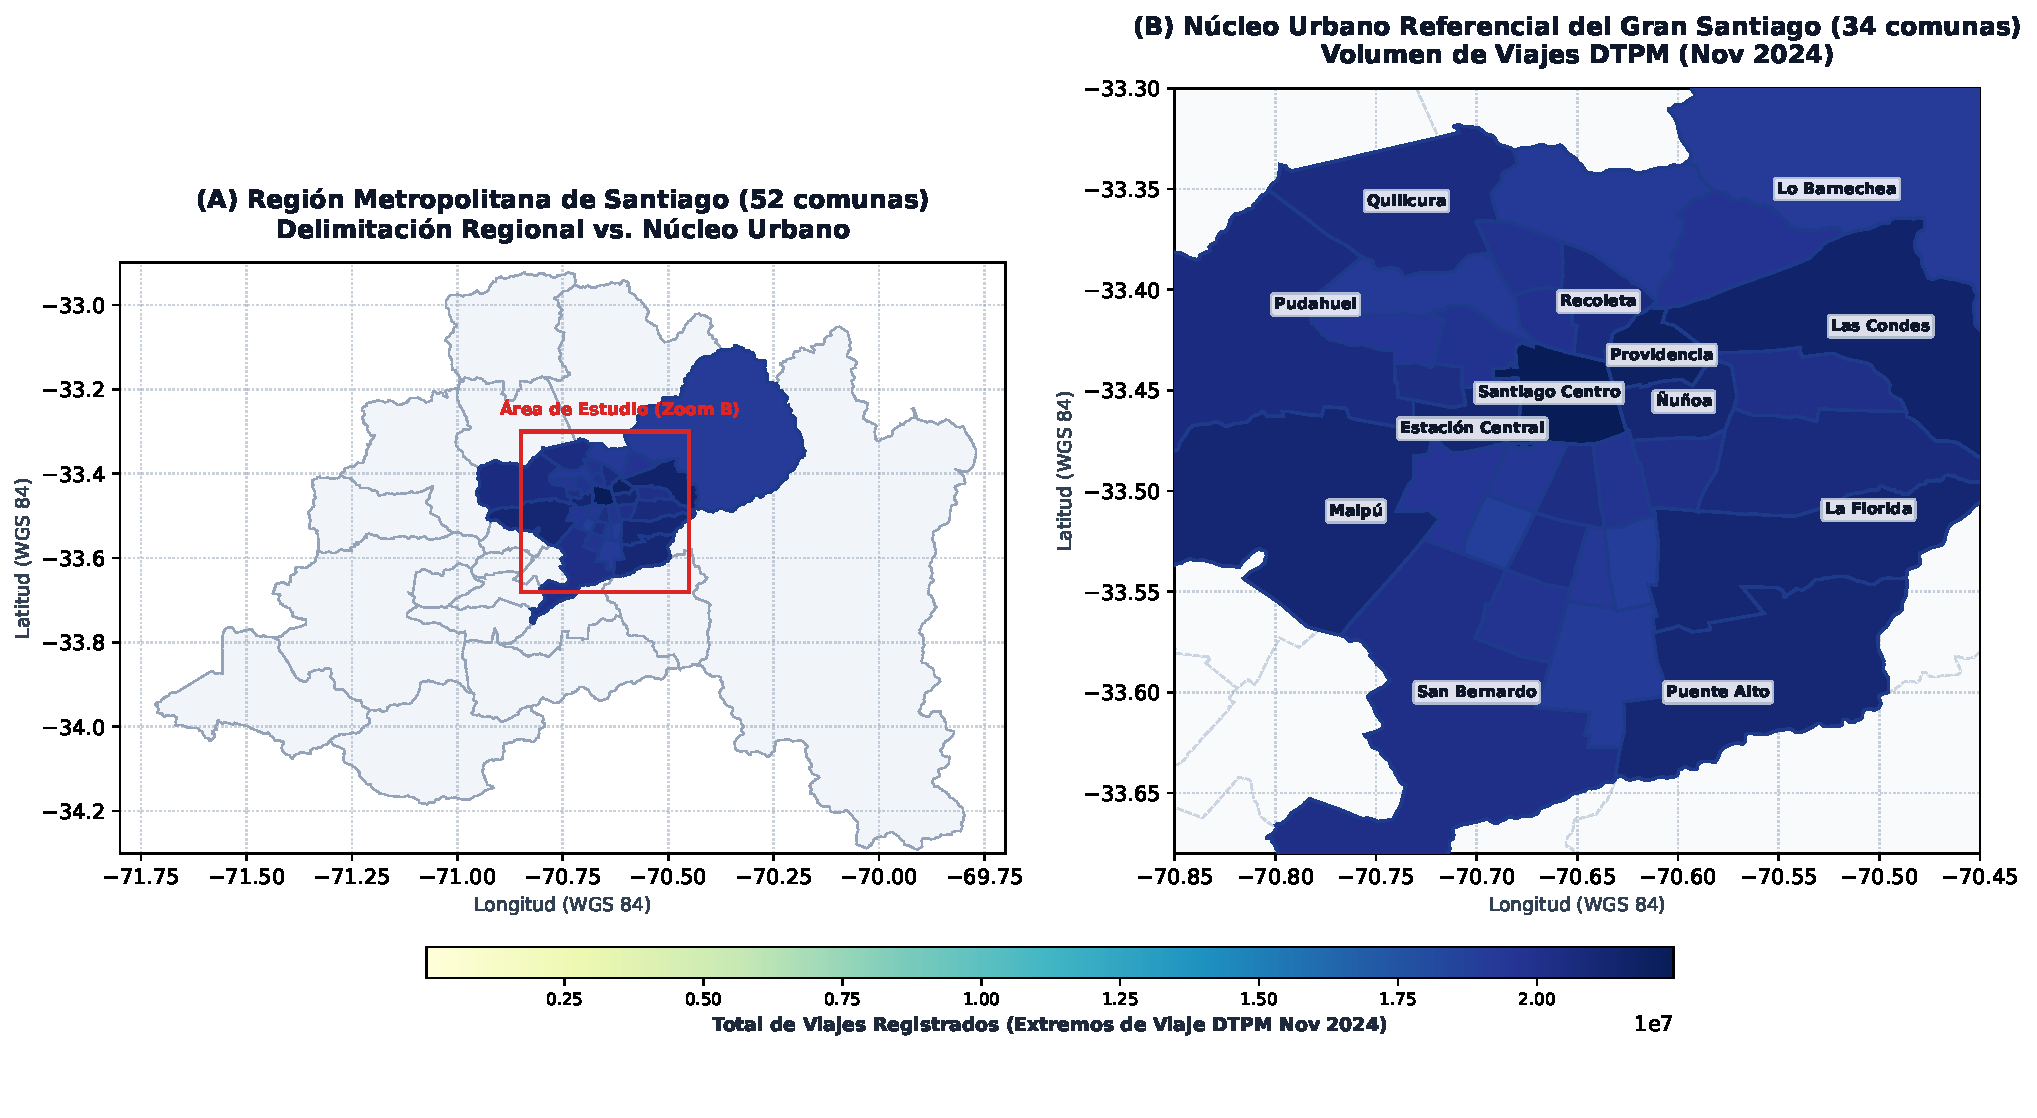
\includegraphics[width=\textwidth]{figures/fig2_delimitacion_gran_santiago_tesis.pdf}
\caption{Delimitación del área de estudio: núcleo urbano referencial de 34 comunas dentro de la Región Metropolitana. Las cifras de la figura corresponden al filtro territorial previo a la exclusión común posterior de tres zonas sin polígono oficial verificable. Fuente: elaboración propia. Los datos territoriales y el procedimiento se describen en esta sección.}
\label{fig:delimitacion_gran_santiago}
\end{figure}

Después del recorte territorial se excluyen, en las tres ramas, los 1.904 viajes que tienen al menos un extremo en las zonas 848, 849 o 852, ya que no disponen de polígono oficial verificable para construir atributos. La cohorte comparativa resultante contiene 60.511.977 viajes y 85.774.522,4070 de masa expandida. Esta exclusión se aplica antes de agregar OD y no se reemplaza mediante geometrías de otra codificación.

La Figura~\ref{fig:serie_diaria_cohorte_final} muestra la cobertura diaria de esta cohorte final. Las 29 fechas disponibles se mantienen con su tipo de día observado; el 30 de noviembre no aparece como cero porque se excluyó por problemas en los archivos de origen.

\begin{figure}[htbp]
\centering
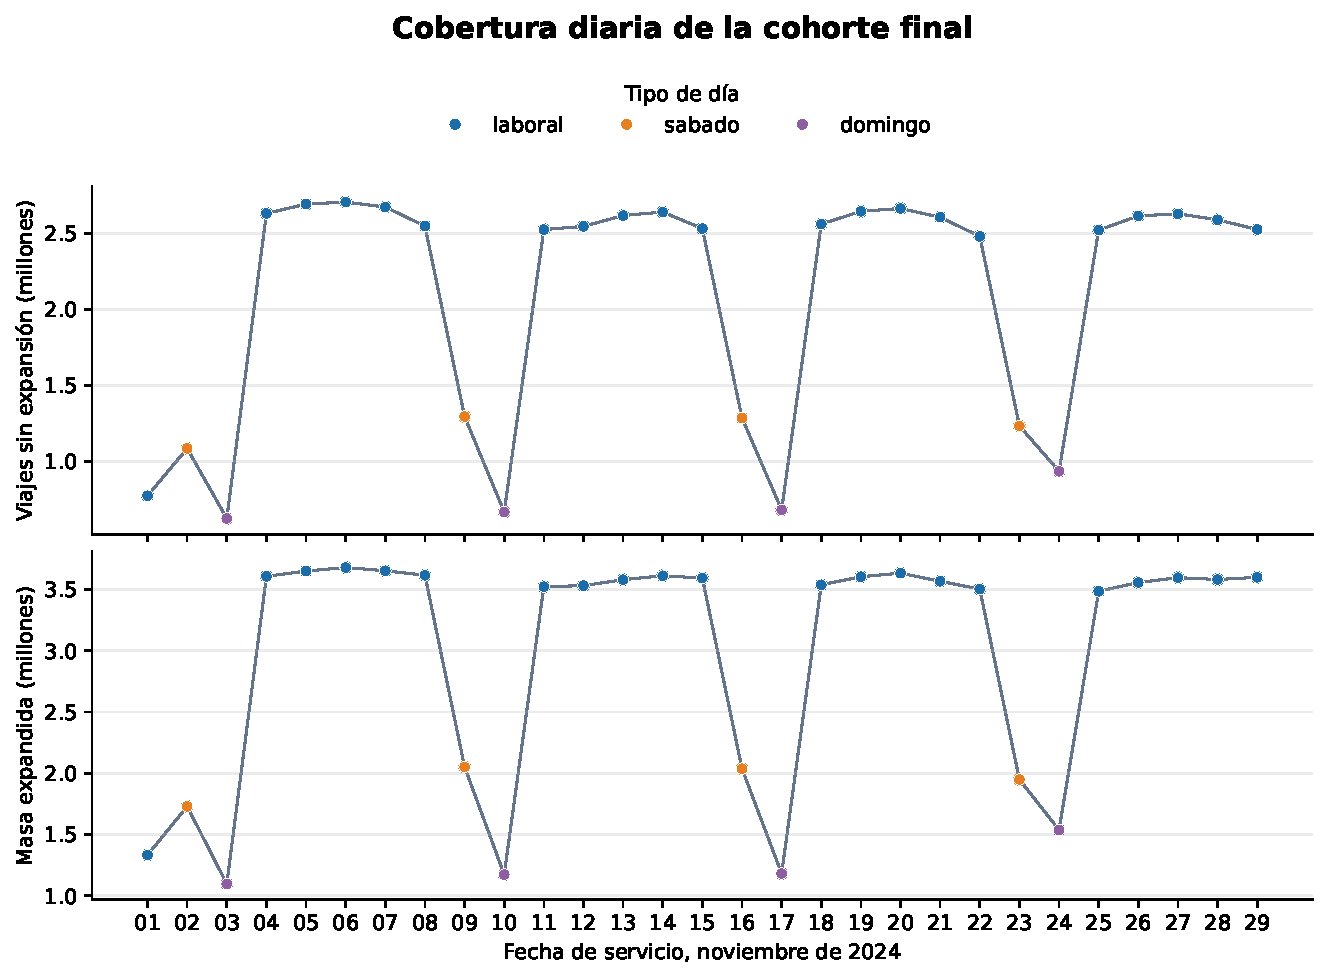
\includegraphics[width=0.93\textwidth]{figures/v05_serie_diaria_cohorte_final.pdf}
\caption{Viajes y masa expandida diarios de la cohorte final. Los puntos distinguen el tipo de día; el OD diario ya está restringido al dominio de 34 comunas y se aplican las exclusiones comunes 848, 849 y 852 en ambos extremos. Se muestran las 29 fechas disponibles, del 1 al 29 de noviembre de 2024; el día 30 no se imputa. Fuente: elaboración propia a partir de los viajes canónicos DTPM.}
\label{fig:serie_diaria_cohorte_final}
\end{figure}

\subsection{Adaptadores espaciales, unidades y \textit{tiles}}
\label{sec:unidades_espaciales}

La rama Zona 777 usa las zonas de origen y destino auditadas en el viaje canónico y la geometría oficial publicada por DTPM. La rama H3 transforma las coordenadas válidas desde EPSG:32719 a WGS84 con \texttt{always\_xy=True} y asigna cada extremo mediante \texttt{latlng\_to\_cell}. La política de borde conserva la celda H3 completa observada: los viajes se recortan por el dominio de estudio, pero las huellas de las celdas no se recortan ni se reparte flujo por superficie.

H3 es un sistema jerárquico de índices geoespaciales. Sus áreas y distancias varían geográficamente, existen pentágonos y la vecindad no puede resumirse como seis vecinos para toda celda. Por ello, H3 no elimina el problema de la unidad espacial modificable (MAUP, por sus siglas en inglés): la comparación trata la discretización espacial como una fuente de sensibilidad empírica. El análisis de factibilidad consideró H3-r3 a H3-r8; H3-r7 y H3-r8 pasaron al piloto junto con Zona 777. La Tabla~\ref{tab:representaciones} presenta las representaciones operativas de la cohorte común, sin inferir superioridad entre ellas.

\begin{table}[htbp]
\centering
\small
\caption{Representaciones espaciales operativas después de la exclusión común. Fuente: elaboración propia.}
\label{tab:representaciones}
\begin{tabularx}{\textwidth}{@{}p{2.1cm}p{2.2cm}p{2.0cm}X@{}}
\toprule
\textbf{Rama} & \textbf{Unidades} & \textbf{Rol} & \textbf{Regla de asignación y alcance} \\
\midrule
Zona 777 & 793 zonas & Referencia zonal & Zonas de origen y destino del viaje canónico; atributos calculados desde la geometría oficial verificable. \\
H3-r7 & 223 celdas & Candidata de escala más agregada & Ambos extremos válidos se asignan directamente a celdas H3; mantiene celdas completas en el borde. \\
H3-r8 & 1.210 celdas & Candidata de mayor detalle & Misma regla de asignación H3 y misma cohorte fuente; su mayor desagregación modifica el soporte OD. \\
\bottomrule
\end{tabularx}
\end{table}

La Figura~\ref{fig:areas_y_soporte_representaciones} complementa esta descripción con las áreas físicas de las unidades y el número de unidades que tienen salida observada en la cohorte completa. Estas diferencias cambian los pares OD evaluables y la masa asignada a prueba; por ello, el CPC se interpreta dentro de cada rama y no como una escala común entre representaciones.

\begin{figure}[htbp]
\centering
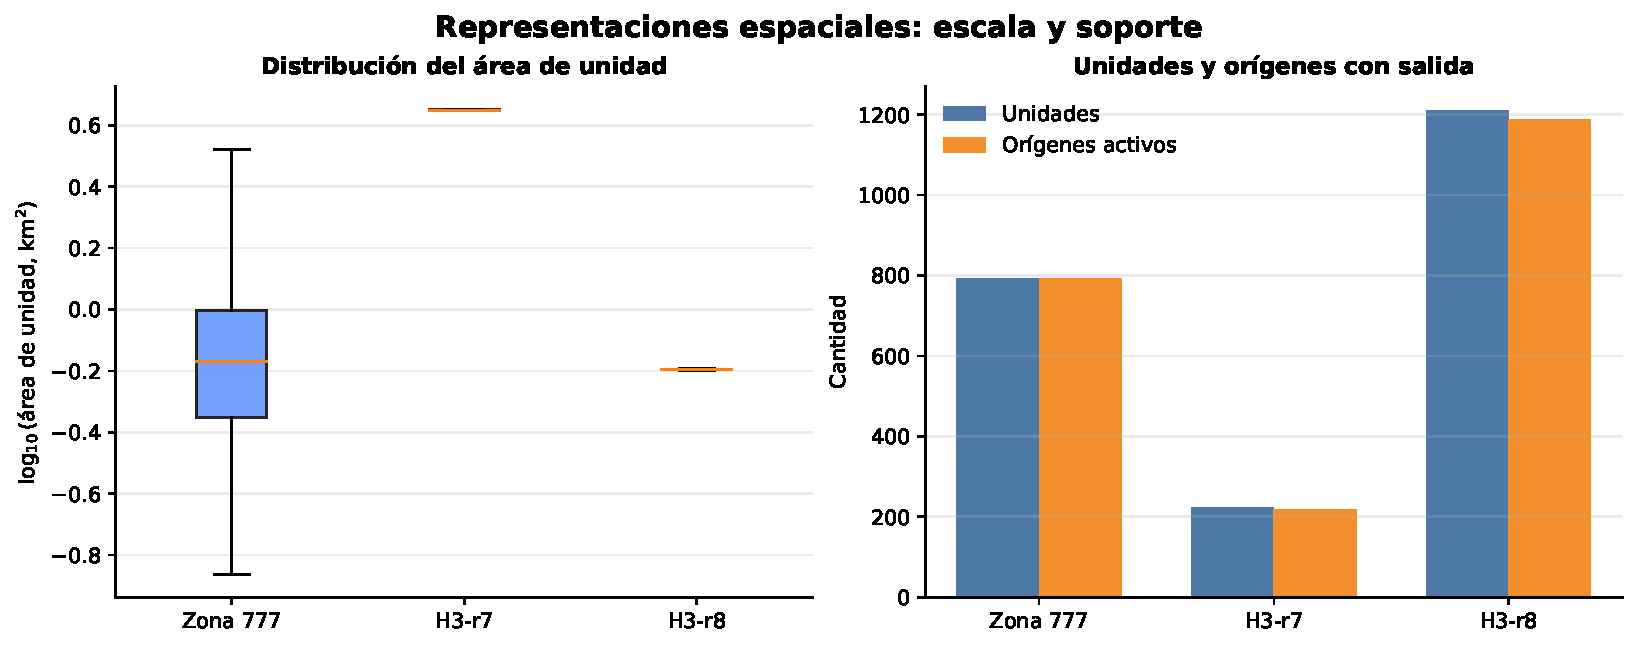
\includegraphics[width=\textwidth]{figures/v07_areas_y_soporte_representaciones.pdf}
\caption{Escalas físicas y soporte de las tres representaciones sobre la misma cohorte final. El panel izquierdo muestra $\log_{10}$ del área de cada unidad en km$^2$; el derecho distingue unidades totales y orígenes con salida observada. La figura no supone igualdad de área ni comparabilidad directa del CPC entre ramas. Fuente: elaboración propia con el contrato territorial y de atributos aprobado y el soporte del experimento mensual.}
\label{fig:areas_y_soporte_representaciones}
\end{figure}

Una zona o celda es una unidad OD. Un \textit{tile} es un bloque mayor, de 15.000 m de lado en EPSG:32719, indexado por $\operatorname{floor}(x/15000)$ y $\operatorname{floor}(y/15000)$. Se fijaron diez \textit{tiles} comunes y una agenda determinista con semilla 20260909: siete para entrenamiento, dos para validación y uno para prueba. La partición se aplica al origen; todos los destinos del dominio de estudio, incluidos los de otros \textit{tiles} o particiones, permanecen candidatos y los flujos cruzados se conservan. La Figura~\ref{fig:objetos_espaciales} distingue estos objetos y evita equiparar un \textit{tile} con una unidad OD.

\begin{figure}[htbp]
\centering
\begin{subfigure}[t]{0.47\textwidth}
\centering
\begin{tikzpicture}[x=0.78cm,y=0.78cm,font=\scriptsize]
    \draw[rounded corners=2pt, thick, fill=blue!4] (0,0) rectangle (5.2,4.0);
    \foreach \x in {0,2.6,5.2} \draw[gray!65] (\x,0) -- (\x,4.0);
    \foreach \y in {0,2,4} \draw[gray!65] (0,\y) -- (5.2,\y);
    \draw[very thick, fill=orange!25] (0.8,0.6) -- (2.2,0.35) -- (3.2,1.0) -- (3.0,2.0) -- (1.7,2.35) -- (0.6,1.7) -- cycle;
    \node[align=center] at (2.6,3.65) {Área de\\estudio};
    \node[align=center] at (1.3,3.0) {\textit{tile}};
    \node[align=center] at (1.9,1.3) {Zona 777\\unidad OD};
\end{tikzpicture}
\caption{Adaptador Zona 777.}
\end{subfigure}
\hfill
\begin{subfigure}[t]{0.47\textwidth}
\centering
\begin{tikzpicture}[x=0.78cm,y=0.78cm,font=\scriptsize]
    \draw[rounded corners=2pt, thick, fill=green!4] (0,0) rectangle (5.2,4.0);
    \foreach \x in {0,2.6,5.2} \draw[gray!65] (\x,0) -- (\x,4.0);
    \foreach \y in {0,2,4} \draw[gray!65] (0,\y) -- (5.2,\y);
    \draw[very thick, fill=cyan!25] (1.25,1.0) -- (1.85,0.65) -- (2.45,1.0) -- (2.45,1.7) -- (1.85,2.05) -- (1.25,1.7) -- cycle;
    \node[align=center] at (2.6,3.65) {Área de\\estudio};
    \node[align=center] at (3.9,3.0) {\textit{tile}};
    \node[align=center] at (1.85,1.35) {Celda\\H3};
\end{tikzpicture}
\caption{Adaptador H3.}
\end{subfigure}
\caption{Escalas espaciales del procedimiento. Cada rama representa el mismo dominio mediante sus propias unidades OD; el \textit{tile} es un bloque de partición mayor y no reemplaza a una zona o celda. Esquema no a escala. Fuente: elaboración propia.}
\label{fig:objetos_espaciales}
\end{figure}

\subsection{Construcción de atributos y vector de entrada}
\label{sec:features_osm}

La configuración principal utiliza 19 variables por ubicación y, para un par OD, forma un vector de 39 entradas: 19 del origen, 19 del destino y una distancia. Incluye densidad de población censal, cinco coberturas de uso de suelo, tres densidades de longitud vial y cinco familias de servicios, cada una medida mediante densidad de puntos y cobertura de áreas. Se conserva una configuración alternativa para diagnóstico, con 20 variables por ubicación y 41 entradas por par, que no reemplaza la configuración principal del piloto.

\begin{equation}
    \mathbf{x}_{ij} = [\mathbf{a}_{i}^{(19)},\, \mathbf{a}_{j}^{(19)},\, d_{ij}],
    \label{eq:vector_entrada}
\end{equation}
donde $\mathbf{a}_{i}$ y $\mathbf{a}_{j}$ contienen los atributos externos de origen y destino, respectivamente, y $d_{ij}$ es la distancia geodésica calculada desde representantes espaciales en WGS84. La población se interpola desde Censo 2024 a las unidades y se divide por su área para construir la densidad de entrada a la red; no se reemplaza por el flujo saliente observado.

Los polígonos y las vías se recortan y unen dentro de cada categoría antes de calcular cobertura o longitud. Los puntos requieren pertenencia estricta a la unidad. Para densidades y tasas se aplica \texttt{log1p}; las coberturas mantienen su escala física antes de estandarizar. Media y desviación estándar se estiman solo con orígenes activos de entrenamiento de cada rama y escenario, y luego se aplican a validación y prueba. Esta regla impide que el conjunto de prueba intervenga en la normalización.

El piloto ajustó esta transformación con los orígenes activos del 5 de noviembre de 2024. En contraste, el experimento principal recalculó y verificó independientemente la normalización mensual a partir de los atributos sin normalizar y de sus propios orígenes de entrenamiento; no reutilizó los parámetros del piloto. Las variables constantes reciben escala uno. Por tanto, una coincidencia de diccionario de atributos no supone que las transformaciones numéricas de ambos escenarios sean intercambiables.

La Figura~\ref{fig:distribuciones_h3_r7} sitúa las escalas de tres magnitudes en H3-r7 antes de la normalización del modelo. El primer histograma condiciona explícitamente en pares OD positivos; el segundo pondera por masa expandida las distancias geodésicas entre centroides, que no representan recorridos de la red; el tercero usa densidad poblacional física, sin las transformaciones aplicadas a la entrada de la red.

\begin{figure}[H]
\centering
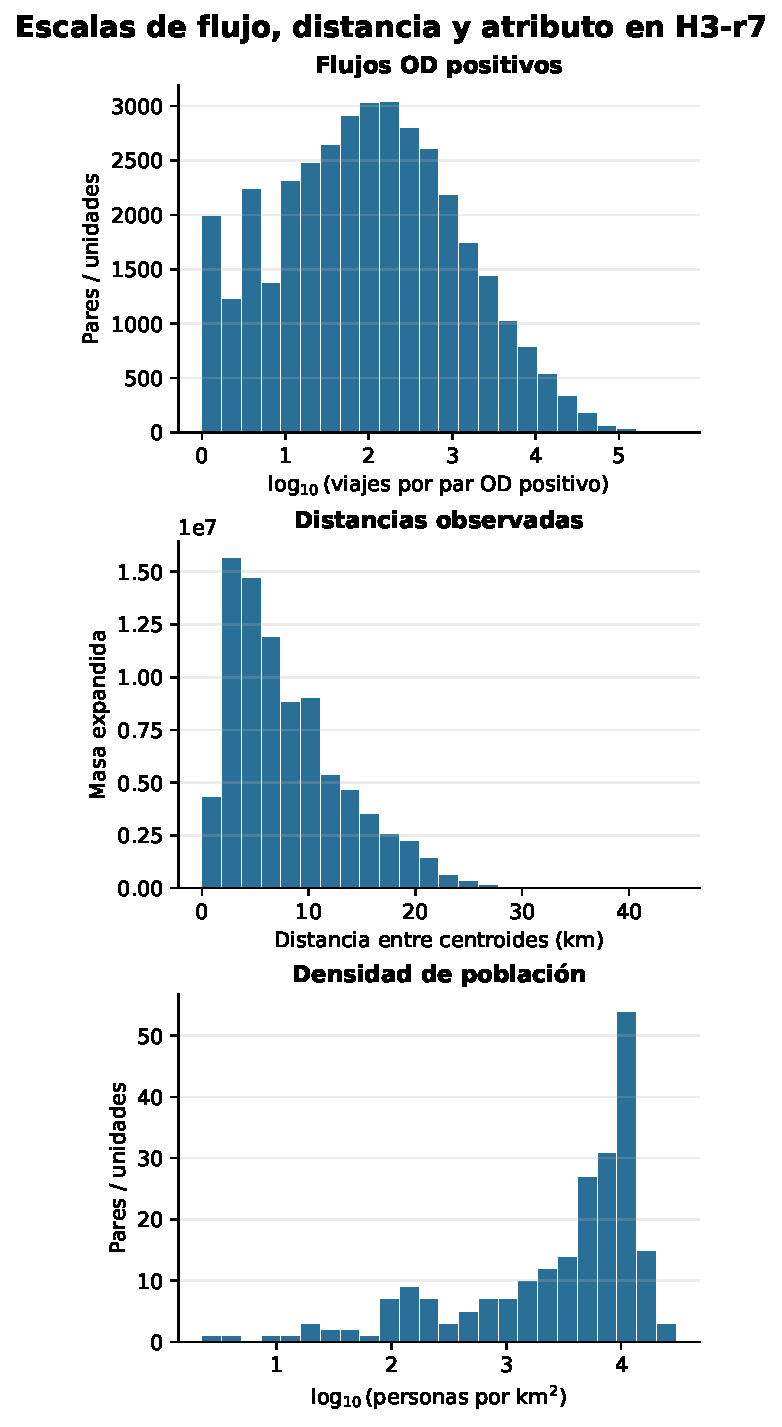
\includegraphics[width=0.60\textwidth]{figures/v06_distribuciones_h3_r7.pdf}
\caption{Escalas de flujo, distancia y densidad poblacional en H3-r7. Los flujos corresponden a pares OD positivos y se expresan en $\log_{10}$ de viajes por par; las distancias entre centroides se agregan con masa expandida; y la densidad poblacional corresponde a personas por km$^2$ antes de la normalización del modelo. Fuente: elaboración propia con la cohorte y los atributos territoriales aprobados.}
\label{fig:distribuciones_h3_r7}
\end{figure}

\subsection{Modelo, muestreo y evaluación}
\label{sec:configuracion_entrenamiento}

\subsubsection{Relación con el modelo gravitatorio}

El \textit{softmax} de una utilidad sistemática $V_{ij}$ define la probabilidad de destino
\begin{equation}
    p_{ij} = \frac{\exp(V_{ij})}{\sum_{k \in \mathcal{D}_i} \exp(V_{ik})},
    \label{eq:logit_dest}
\end{equation}
donde $\mathcal{D}_i$ es el soporte de destinos permitido para el origen $i$. Si $V_{ij}=\beta_1\ln(P_j)+\beta_2\ln(d_{ij})$, el \textit{softmax} induce una forma de potencia $P_j^{\beta_1}d_{ij}^{\beta_2}$; no induce una disuasión exponencial. Una forma gravitatoria exponencial requiere, por ejemplo, una utilidad coherente $V_{ij}=\alpha\ln(P_j)-\beta d_{ij}$ \cite{mcfadden1974conditional,ortuzar2011modelling}.

\textit{Deep Gravity} reemplaza la utilidad lineal por una función no lineal aprendida $f_\theta(\mathbf{x}_{ij})$. El teorema de aproximación universal respalda una capacidad de representación bajo sus supuestos, pero no garantiza que una arquitectura concreta se optimice, generalice o supere a un \textit{baseline} con datos finitos \cite{hornik1991approximation}.

\subsubsection{Arquitectura, soporte y pérdida}

La implementación efectiva conserva 15 capas ocultas: cinco de ancho 256 y diez de ancho 128, con activaciones LeakyReLU. No usa BatchNorm y el \textit{dropout} efectivo es 0,0 en la ruta vigente. La capa final produce un \textit{score} por destino candidato. La arquitectura heredada y la corrida técnica de Nueva York se mantienen como antecedentes de compatibilidad, no como demostración de desempeño científico para Santiago.

El muestreador general permite limitar el número de destinos por origen, sin reposición, y reservar una fracción de candidatos con flujo positivo. Los candidatos restantes se eligen uniformemente entre los disponibles, por lo que pueden incluir otros destinos con flujo positivo. Esa opción no se utilizó en el piloto ni en el experimento mensual: tanto el entrenamiento como la evaluación usaron el soporte completo de destinos de cada representación. Los destinos de todo el dominio metropolitano permanecieron disponibles aunque correspondieran a otro \textit{tile} o partición.

La pérdida es la log-verosimilitud multinomial negativa ponderada por la masa elegida:
\begin{equation}
    \mathcal{L} = -\sum_{i}\sum_{j \in \mathcal{D}_i} y_{ij}\log p_{ij}.
    \label{eq:perdida_multinomial_santiago}
\end{equation}
Para conteos enteros, minimizar esta expresión equivale a maximizar la log-verosimilitud multinomial, salvo constantes independientes del modelo. Con masa expandida fraccionaria, se interpreta como una pérdida multinomial ponderada, con el soporte de destinos y los pesos definidos para el análisis. Su relación con la formulación de entropía de Wilson es conceptual y requiere restricciones adicionales; no se identifica automáticamente con maximizar la entropía de Wilson \cite{wilson1970entropy}.

\subsubsection{Modelos de referencia, particiones y métricas}

Las tres referencias se ajustan solamente con los flujos cuyos orígenes pertenecen a entrenamiento y se evalúan sobre los mismos orígenes, destinos y masa que la red dentro de cada rama. La referencia uniforme asigna $1/|\mathcal{D}|$ a cada destino del soporte. La referencia de atracción usa la masa expandida recibida durante entrenamiento:
\begin{equation}
    \widehat y_{ij}=O_i\,
    \frac{A_j^{\mathrm{train}}+\lambda}
    {\sum_{k\in\mathcal{D}}A_k^{\mathrm{train}}+\lambda|\mathcal{D}|},
    \qquad \lambda=1.
    \label{eq:baseline_atraccion}
\end{equation}
donde $A_j^{\mathrm{train}}$ es la masa que llega a $j$ desde los orígenes de entrenamiento, $\mathcal{D}$ es el soporte completo de destinos de la rama y $O_i$ es el flujo saliente observado del origen que se evalúa. El pseudoconteo $\lambda$ corresponde a una unidad de masa por destino. Esta referencia distribuye una salida observada; no es población, ni un atributo de la red, ni una estimación de la generación de viajes.

En el modelo gravitatorio exponencial, la utilidad se calcula como
\begin{equation}
    V_{ij}=\alpha\ln(1+P_j)+\beta d_{ij},\qquad \alpha\geq0,\quad\beta\leq0,
    \label{eq:baseline_exponencial}
\end{equation}
donde $P_j$ es la población total interpolada, recuperada multiplicando la densidad censal por el área de la unidad, y $d_{ij}$ es la distancia esférica en kilómetros. Los parámetros se ajustan exclusivamente con los flujos de entrenamiento mediante una pérdida multinomial ponderada y L-BFGS-B, inicializado en $(1,-0{,}1)$, con un máximo de 500 iteraciones, $\textit{ftol}=10^{-12}$ y $\textit{gtol}=10^{-8}$; se imponen $\alpha\geq0$ y $\beta\leq0$. Esta variable del modelo de referencia se distingue de la densidad de población transformada y estandarizada que recibe la red. La distancia intrazonal o intracelda es cero, valor admisible en la disuasión exponencial.

El piloto verificó la comparación contra estas tres referencias en el mismo soporte de cada rama. El \textit{checkpoint} se selecciona por CPC de validación; la prueba se ejecuta después y no ajusta parámetros. La configuración del piloto usa RMSprop, tasa de aprendizaje $5\times10^{-6}$, momento 0,9, lotes de ocho orígenes y 15 épocas. Estos valores son una configuración de piloto registrada, no una selección definitiva de hiperparámetros para el experimento mensual.

La métrica principal es
\begin{equation}
    \mathrm{CPC}=\frac{2\sum_{ij}\min(T_{ij},\widehat{T}_{ij})}{\sum_{ij}T_{ij}+\sum_{ij}\widehat{T}_{ij}}.
    \label{eq:cpc_santiago}
\end{equation}
Se guardan numerador y ambas masas por origen para agregar CPC global y por \textit{tile} sobre el mismo soporte. Las medias por origen, por todos los \textit{tiles} y condicionadas a CPC positivo se reportan separadamente. El piloto de Santiago confirma que el procedimiento se puede ejecutar y repetir con tres semillas, pero una comparación directa de CPC entre resoluciones no demuestra por sí sola superioridad de H3: cambian la agregación, los representantes espaciales y la masa de prueba entre ramas.

\subsubsection{Piloto y experimento mensual}

El piloto utilizó el martes 5 de noviembre de 2024. Incluyó diagnósticos en una muestra, en el día completo y en tres ventanas horarias, y nueve corridas estables del día completo: tres ramas y las semillas 20260909, 20260910 y 20260911. Cada corrida estable se entrenó durante 15 épocas; el mejor \textit{checkpoint} de validación se conservó y se evaluó posteriormente en prueba. Las ventanas y el número de épocas sirvieron para comprobar la factibilidad y estabilidad iniciales, no para establecer convergencia, ajustar hiperparámetros ni generalizar el comportamiento de un día al período mensual.

El experimento principal agrega las 29 fechas disponibles entre el 1 y el 29 de noviembre de 2024; el día 30 se excluye por problemas en los archivos y no se imputa. Se entrenaron nueve modelos desde inicializaciones nuevas: las tres ramas y las mismas tres semillas. La red, el soporte completo y la pérdida fueron los descritos antes. El optimizador fue RMSprop con tasa $5\times10^{-6}$, momento 0,9, $\alpha=0{,}99$, $\epsilon=10^{-8}$, sin decaimiento de pesos ni centrado; se usaron lotes de ocho orígenes en orden estable y sin barajado. Las corridas se ejecutaron secuencialmente en CPU con cuatro hilos. Cada época evaluó todos los orígenes de validación.

La selección del \textit{checkpoint} y la parada anticipada obedecieron a reglas diferentes. Se conservó el \textit{checkpoint} con el mayor CPC global de validación entre todas las épocas ejecutadas y, ante un empate exacto, el primero. Para la parada, la primera época de validación inicializó una referencia significativa; esta se actualizó solo si el CPC posterior era estrictamente mayor que la referencia más $0{,}0001$. Tras un mínimo de 50 épocas, la corrida se detenía cuando acumulaba 30 épocas sin esa mejora significativa. El límite inicial fue 200 épocas: alcanzarlo sin meseta no se interpretaba como convergencia ni autorizaba una extensión automática.

Dos corridas alcanzaron dicho límite y recibieron una autorización previa a la prueba para continuar, sin reinicializar ni alterar datos, particiones, arquitectura, optimizador, métrica o regla de selección. La continuación elevó el máximo a 300 épocas para Zona 777 con semilla 20260909 y H3-r8 con semilla 20260910. Ambas cerraron posteriormente por la misma regla de meseta, en las épocas 226 y 218, respectivamente; sus \textit{checkpoints} seleccionados permanecieron en las épocas 196 y 188. Las demás corridas cerraron con la configuración inicial. La prueba se liberó una sola vez después de congelar las fuentes, las decisiones de validación y los \textit{checkpoints} seleccionados; no intervino en la elección de época, semilla, parámetros o representación.

Como análisis de sensibilidad de la evaluación, las probabilidades ya congeladas se aplicaron también a los conteos OD sin expansión y se reescalaron por el flujo saliente no expandido de cada origen. El CPC resultante es secundario: no implica reentrenamiento sin pesos, nueva selección ni un nuevo ajuste de los modelos de referencia, cuyos parámetros se obtuvieron con la masa expandida.

\subsection{Análisis complementario de atribuciones predictivas}

Después de congelar los modelos mensuales se evaluó la viabilidad de explicar la log-probabilidad condicional de un destino dentro del soporte completo de cada origen. Los representantes se escogieron por la mediana del CPC de validación de cada rama, sin usar el CPC de prueba ni la apariencia de una atribución. Las referencias se construyeron exclusivamente con orígenes de entrenamiento de la rama correspondiente; la función explicada, la muestra y los controles se fijaron antes de cada ejecución. Se ensayaron gradientes integrados con cuadratura Gauss--Legendre \cite{sundararajan2017axiomatic}, SHAP por permutaciones agrupadas y valores de Shapley exactos para grupos jerárquicos \cite{lundberg2017shap}. En todos los casos las atribuciones se definieron como sensibilidad predictiva dependiente de la referencia, no como efectos causales.

Las tres aproximaciones se evaluaron contra controles de integridad, coincidencia entre el adaptador y la salida del modelo, finitud, convergencia o eficiencia según el método, repetibilidad y estabilidad frente a fondos independientes. Los gradientes integrados no acreditaron completitud para una consulta crítica aun con 4.096 nodos. El método por permutaciones no acreditó estabilidad entre fondos en dos de tres semillas de su primera consulta obligatoria. El método exacto jerárquico acreditó una primera consulta a 24 fondos, pero otra consulta crítica no acreditó la estabilidad de los tres supergrupos a 24 ni a 48 fondos. En consecuencia, ninguna aproximación superó todos los controles requeridos para publicar atribuciones. No se presentan rankings, atribuciones, figuras SHAP ni casos locales; los registros técnicos se conservan como respaldo reproducible y el desenlace se desarrolla en el Capítulo~5.

\subsection{Reproducibilidad, alcances y limitaciones}
\label{sec:alcances}

Cada ejecución conserva configuración efectiva, semillas, versiones, hashes de entradas y código, particiones, métricas y \textit{checkpoint} en un directorio exclusivo. Los productos de datos, las especificaciones de procesamiento y los registros de ejecución permiten verificar la conservación de masa y reconstruir la procedencia de cada corrida. La prueba espacial se mantiene reservada durante la selección; el conjunto de prueba no participa en la normalización ni en el ajuste de hiperparámetros.

El alcance se limita a la movilidad observable en DTPM durante las 29 fechas disponibles de noviembre de 2024 y al dominio de estudio de 34 comunas. No representa todos los modos urbanos, no predice la generación total de viajes por origen ni fechas futuras. El piloto no acredita por sí mismo generalización temporal al período mensual. A su vez, el agregado mensual incluye el 5 de noviembre y reutiliza la misma geografía de prueba, por lo que no constituye una prueba enteramente nueva e independiente del piloto. Las tres semillas caracterizan variación de inicialización bajo una sola partición espacial, no incertidumbre espacial o poblacional. La instantánea OSM antecede a los viajes y su cobertura no equivale a presencia real de servicios; la interpolación areal del Censo 2024 supone distribución uniforme dentro de cada geometría censal. Además, la exclusión de las zonas sin polígono, la decisión de discretización y las diferencias de agregación espacial condicionan toda interpretación comparativa.

El resultado del análisis complementario de explicabilidad limita la interpretación de las características territoriales: bajo las configuraciones ensayadas no fue posible obtener atribuciones suficientemente estables para una interpretación sustantiva. Esta limitación no altera las métricas predictivas ni las comparaciones con referencias, que se fundamentan en su propio protocolo de evaluación.

\newpage
\secnumbersection{VALIDACIÓN DE LA SOLUCIÓN}
\label{sec:cap5}

La validación distingue el piloto del 5 de noviembre de 2024 del experimento mensual congelado. Este último agrega las 29 fechas disponibles entre el 1 y el 29 de noviembre, conserva tres inicializaciones por representación y libera la prueba una sola vez después de seleccionar los \textit{checkpoints} con validación. Las métricas se calculan con la definición de CPC de la ecuación~\eqref{eq:cpc_santiago}; la comparación sustantiva se realiza entre modelos que comparten soporte dentro de cada rama.

\subsection{Piloto como validación preliminar}
\label{sec:piloto_preliminar}

El piloto se realizó sobre el martes 5 de noviembre de 2024 para comprobar el recorrido de datos, el entrenamiento, la selección por validación y la evaluación sobre el soporte completo de destinos. Incluyó 15 corridas diagnósticas y nueve entrenamientos estables del día completo, con tres representaciones espaciales y tres inicializaciones por representación. Cada entrenamiento se limitó a 15 épocas. Las ventanas horarias tuvieron un propósito diagnóstico y no se usaron para establecer una comparación final entre períodos.

En la prueba del piloto, el CPC medio de Deep Gravity fue 0,4920 en Zona 777, 0,7172 en H3-r7 y 0,5623 en H3-r8. Las desviaciones estándar muestrales entre las tres inicializaciones fueron 0,0045, 0,0021 y 0,0017, respectivamente. Dentro de cada representación, el modelo de atracción entrenado obtuvo los CPC más altos, con 0,6457, 0,7764 y 0,6669. Estos resultados acreditan la factibilidad del procedimiento y muestran que la comparación con referencias debe conservarse en el experimento mensual; no acreditan convergencia, ajuste óptimo ni generalización temporal.

El experimento mensual no se interpreta como una réplica completamente independiente del piloto. Comparte la geografía de prueba y contiene el 5 de noviembre. La diferencia entre ambos escenarios reúne cambios de período, normalización, volumen de datos y presupuesto de entrenamiento, de modo que no puede atribuirse a un único factor.

\subsection{Soporte de prueba y caracterización espacial}
\label{sec:soporte_prueba}

El experimento principal agrega la cohorte final de 60.511.977 viajes, con masa expandida de 85.774.522,4070, observados entre el 1 y el 29 de noviembre de 2024. La Tabla~\ref{tab:soporte_prueba} hace explícitos los denominadores de prueba. Aunque la cohorte fuente es común, cada adaptador espacial asigna unidades, pares candidatos y masa de prueba propios. La evaluación mantiene el soporte completo de destinos para cada origen de prueba; las unidades sin origen asignado no se convierten en observaciones inactivas ni se eliminan del conjunto de destinos.

\begin{table}[htbp]
\centering
\small
\renewcommand{\arraystretch}{1.12}
\caption{Soporte de prueba por representación. Los pares positivos y su densidad se calculan sobre los pares candidatos indicados. La masa observada usa el factor de expansión; los orígenes activos e inactivos se refieren a la partición de prueba. Fuente: elaboración propia a partir de la tabla de soporte del experimento mensual.}
\label{tab:soporte_prueba}
\resizebox{\textwidth}{!}{%
\begin{tabular}{@{}lrrrrrr@{}}
\toprule
\textbf{Rama} & \textbf{Unid.} & \textbf{Orígenes} & \textbf{Sin asignar} & \textbf{Destinos} & \textbf{Pares candidatos} & \textbf{Masa exp.} \\
\midrule
Zona 777 & 793 & 101 (101/0) & 0 & 793 & 80.093 (61.132; 76,3\%) & 16,11 M \\
H3-r7 & 223 & 32 (32/0) & 5 & 223 & 7.136 (5.552; 77,8\%) & 17,39 M \\
H3-r8 & 1.210 & 189 (189/0) & 21 & 1.210 & 228.690 (99.374; 43,5\%) & 15,80 M \\
\bottomrule
\end{tabular}
}
\end{table}

En la columna de orígenes, el par entre paréntesis corresponde a activos/inactivos; en la columna de pares, el paréntesis contiene pares OD positivos y su densidad. La masa expandida se expresa en millones de unidades de masa observada. Los desgloses por origen y \textit{tile} se conservan como respaldo reproducible. La densidad de pares OD positivos fue 76,33\% en Zona 777, 77,80\% en H3-r7 y 43,45\% en H3-r8.

Las representaciones se construyen a partir de la misma cohorte, pero no comparten una partición de prueba idéntica una vez que cada viaje se asigna a una unidad espacial. Cambian el número de destinos por origen, los pares candidatos, la densidad OD y la masa de prueba. Por esta razón, el CPC no permite ordenar las tres representaciones como si fueran mediciones de una misma tarea. La comparación principal se realiza dentro de cada representación, contra referencias evaluadas en el mismo soporte.

La Figura~\ref{fig:concentracion_zona777} caracteriza la distribución espacial de la masa expandida en la rama zonal. Sus dos paneles usan la misma cohorte final y expresan concentración por superficie; no son mapas de error ni una medida de desempeño predictivo.

\begin{figure}[H]
\centering
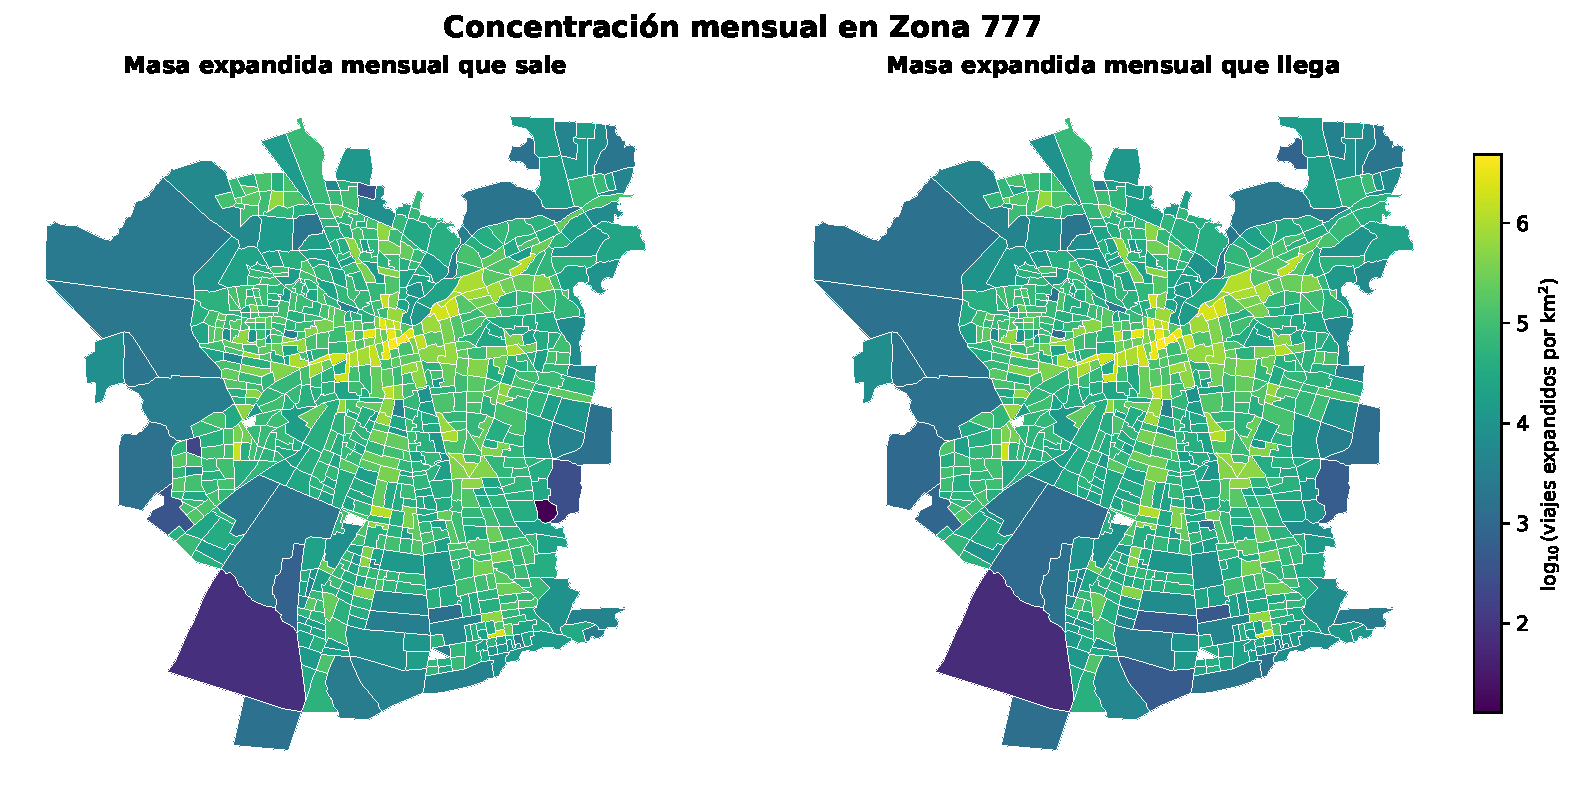
\includegraphics[width=\textwidth]{figures/v04_concentracion_origen_destino_zona777.pdf}
\caption{Concentración mensual de la masa expandida que sale y llega por km$^2$ en Zona 777. Cada panel usa la cohorte final de 60.511.977 viajes, del 1 al 29 de noviembre de 2024; los colores muestran $\log_{10}$ de masa expandida por km$^2$. Fuente: elaboración propia con datos DTPM y geometría oficial Zona 777.}
\label{fig:concentracion_zona777}
\end{figure}

\subsection{Resultados globales en prueba}
\label{sec:resultados_globales_prueba}

La Tabla~\ref{tab:resultados_prueba} reúne el CPC global de prueba con peso expandido. Deep Gravity se resume mediante media, desviación estándar muestral y rango de las tres inicializaciones; los modelos de referencia son deterministas y se ajustan solamente con los flujos de entrenamiento de la rama correspondiente. Las cifras no ordenan las representaciones entre sí, porque cambian las unidades, el soporte y la masa de prueba.

\begin{table}[H]
\centering
\small
\renewcommand{\arraystretch}{1.15}
\caption{CPC global de prueba con peso expandido y salida condicionada al flujo saliente observado. Deep Gravity se resume con tres inicializaciones independientes; DE es la desviación estándar muestral. Uniforme, atracción entrenada y gravedad exponencial se calculan una vez por rama sobre el mismo soporte de prueba. Fuente: elaboración propia a partir de los resultados mensuales congelados.}
\label{tab:resultados_prueba}
\resizebox{\textwidth}{!}{%
\begin{tabular}{@{}lccccc@{}}
\toprule
\textbf{Rama} & \textbf{Deep Gravity} & \textbf{Rango} & \textbf{Uniforme} & \textbf{Atracción} & \textbf{Gravedad exp.} \\
\midrule
Zona 777 & 0,5609 $\pm$ 0,0062 & 0,5537--0,5647 & 0,2992 & 0,6574 & 0,3819 \\
H3-r7 & 0,7722 $\pm$ 0,0060 & 0,7671--0,7787 & 0,3702 & 0,7757 & 0,6153 \\
H3-r8 & 0,6079 $\pm$ 0,0047 & 0,6046--0,6133 & 0,2611 & 0,6867 & 0,3777 \\
\bottomrule
\end{tabular}
}
\end{table}

La Figura~\ref{fig:cpc_semillas_referencias} muestra los mismos resultados sin ocultar las tres semillas. Los cuadrados corresponden a los modelos de referencia y los círculos a inicializaciones de Deep Gravity; la lectura válida sigue siendo dentro de cada panel o rama.

\begin{figure}[H]
\centering
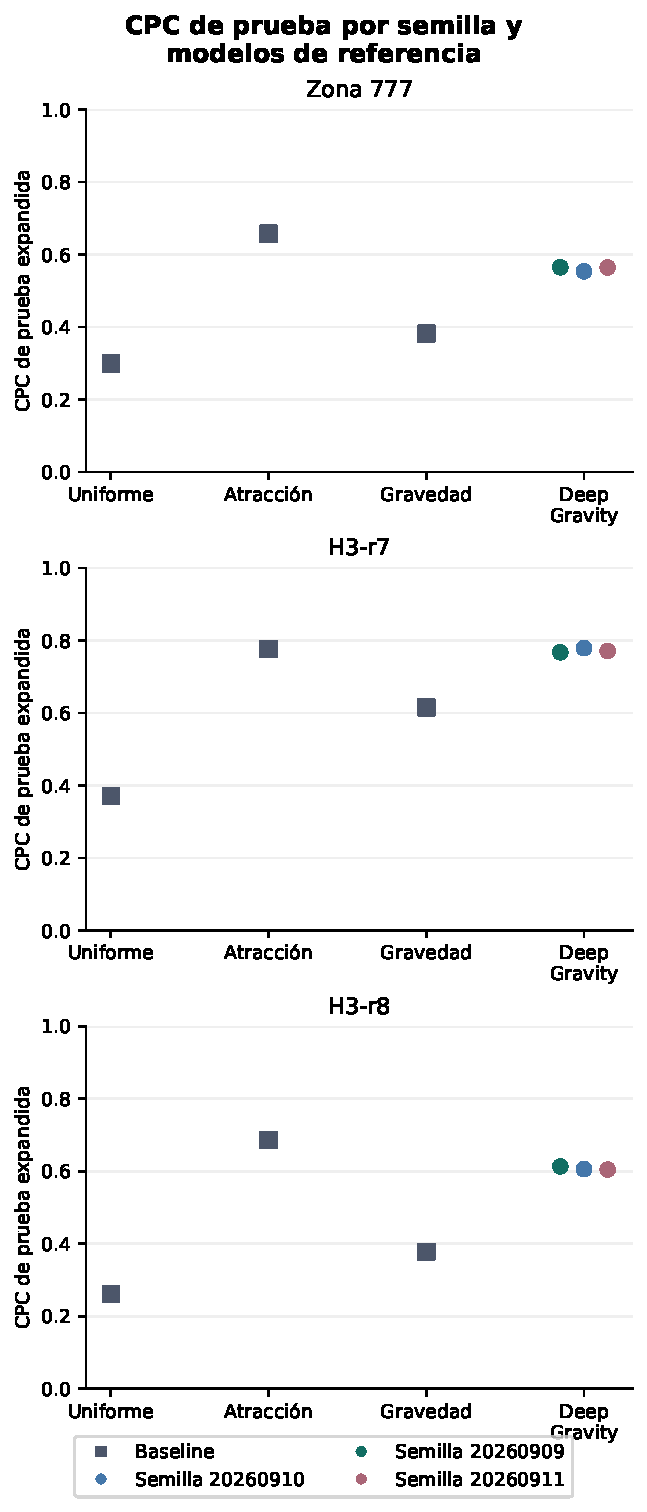
\includegraphics[width=0.45\textwidth]{figures/cpc_semillas_y_referencias.pdf}
\caption{CPC de prueba expandida por semilla y modelos de referencia. Cada panel corresponde a una representación y mantiene su propio soporte de destinos; los cuadrados son referencias deterministas y los círculos son las semillas 20260909, 20260910 y 20260911 de Deep Gravity. Fuente: elaboración propia a partir de las métricas globales del experimento mensual.}
\label{fig:cpc_semillas_referencias}
\end{figure}

\FloatBarrier

Deep Gravity superó las referencias uniforme y de gravedad exponencial en las tres representaciones. En Zona 777, el CPC medio fue 0,5609, frente a 0,2992 para la referencia uniforme y 0,3819 para la referencia gravitacional. En H3-r7, los valores fueron 0,7722, 0,3702 y 0,6153. En H3-r8, fueron 0,6079, 0,2611 y 0,3777. La magnitud de esas diferencias sólo se interpreta dentro de cada representación porque el soporte y la agregación cambian entre ellas.

La referencia de atracción entrenada superó la media de Deep Gravity en las tres representaciones: 0,6574 frente a 0,5609 en Zona 777, 0,7757 frente a 0,7722 en H3-r7 y 0,6867 frente a 0,6079 en H3-r8. La diferencia fue particularmente pequeña en H3-r7, donde una inicialización de Deep Gravity alcanzó 0,7787 y superó individualmente el valor de atracción. Esa observación no altera el resumen de las tres inicializaciones ni autoriza seleccionar una semilla a partir de prueba. El resultado principal es que, bajo esta configuración, la red mejora sobre las referencias uniforme y gravitacional, pero no supera en promedio a la referencia de atracción ajustada con entrenamiento.

La conservación de masa se verificó para todos los orígenes de prueba. El mayor error absoluto por origen fue $1{,}863\times10^{-9}$. Este control confirma que la conversión de probabilidades en flujos preserva el flujo saliente observado, sin convertir la tarea en un modelo de generación total de viajes.

\subsection{Trayectorias y selección por validación}
\label{sec:trayectorias_validacion}

La Figura~\ref{fig:trayectorias_mensuales} conserva las trayectorias de las nueve corridas y permite distinguir la pérdida de entrenamiento del CPC de validación utilizado para elegir los \textit{checkpoints}. La línea vertical discontinua marca el límite inicial de 200 épocas; solo Zona 777--20260909 y H3-r8--20260910 continuaron mediante las extensiones autorizadas, sin alterar datos, arquitectura, optimizador, particiones o regla de selección.

\begin{figure}[htbp]
\centering
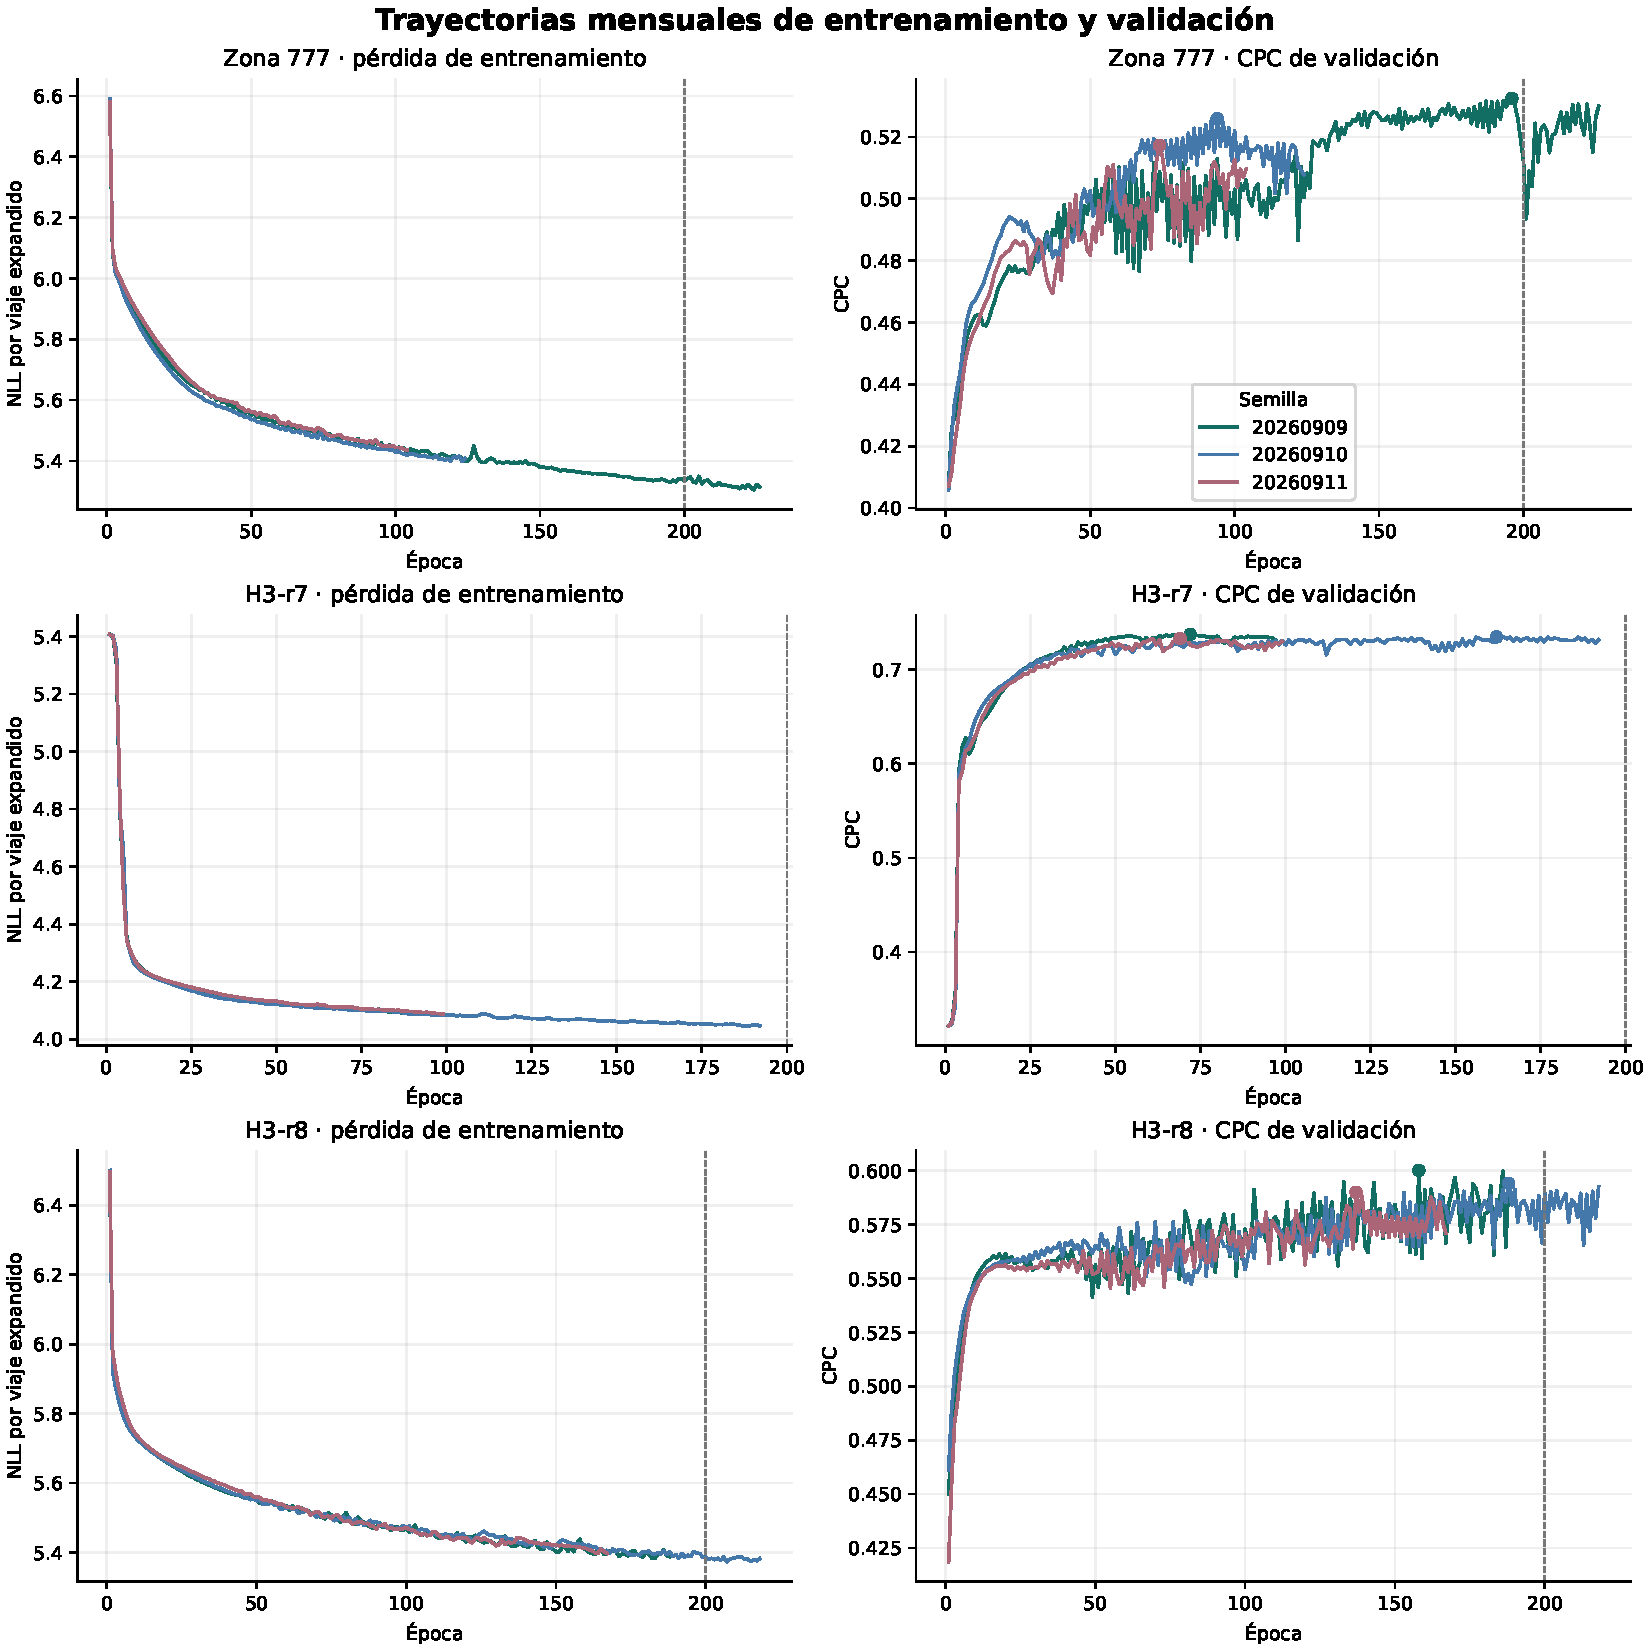
\includegraphics[width=0.96\textwidth]{figures/trayectorias_entrenamiento_validacion.pdf}
\caption{Trayectorias mensuales de pérdida de entrenamiento y CPC global de validación para las tres semillas de cada rama. La pérdida se expresa como NLL por viaje expandido; los puntos destacados marcan los \textit{checkpoints} seleccionados por CPC de validación y la línea discontinua señala la época 200. Fuente: elaboración propia a partir de las trayectorias del experimento mensual.}
\label{fig:trayectorias_mensuales}
\end{figure}

Todas las corridas cerraron por meseta de validación. Las dos extensiones no alteraron datos, particiones, arquitectura, optimizador ni regla de selección. La corrida de Zona 777 con semilla 20260909 cerró en la época 226 y mantuvo como \textit{checkpoint} seleccionado la época 196. La corrida de H3-r8 con semilla 20260910 cerró en la época 218 y mantuvo la época 188. Las restantes siete corridas cerraron sin extensión.

Los rangos de CPC de prueba entre las tres inicializaciones fueron 0,0110 en Zona 777, 0,0117 en H3-r7 y 0,0087 en H3-r8. Ninguno excedió la alerta protocolaria de 0,05. Esta dispersión describe la variación asociada a la inicialización y al entrenamiento bajo una partición espacial fija. No estima incertidumbre poblacional, variación entre particiones ni significación estadística.

Una verificación independiente volvió a evaluar un \textit{checkpoint} seleccionado por validación en cada representación. Las diferencias absolutas de CPC fueron inferiores a $10^{-6}$, con soporte completo de destinos. Esta comprobación respalda la consistencia técnica de la evaluación congelada, pero no equivale a una validación científica en otra ciudad, período o partición espacial.

\subsection{Sensibilidad al peso de evaluación}
\label{sec:sensibilidad_peso}

La Figura~\ref{fig:sensibilidad_pesos} contrasta el CPC calculado con masa expandida y con conteos sin expansión. En ambos ejes se aplican las mismas probabilidades ya congeladas y cada origen se reescala con su respectivo flujo saliente; el eje sin expansión no corresponde a un reentrenamiento ni a una nueva selección de modelos. La diagonal indica igualdad entre ambas evaluaciones.

\begin{figure}[htbp]
\centering
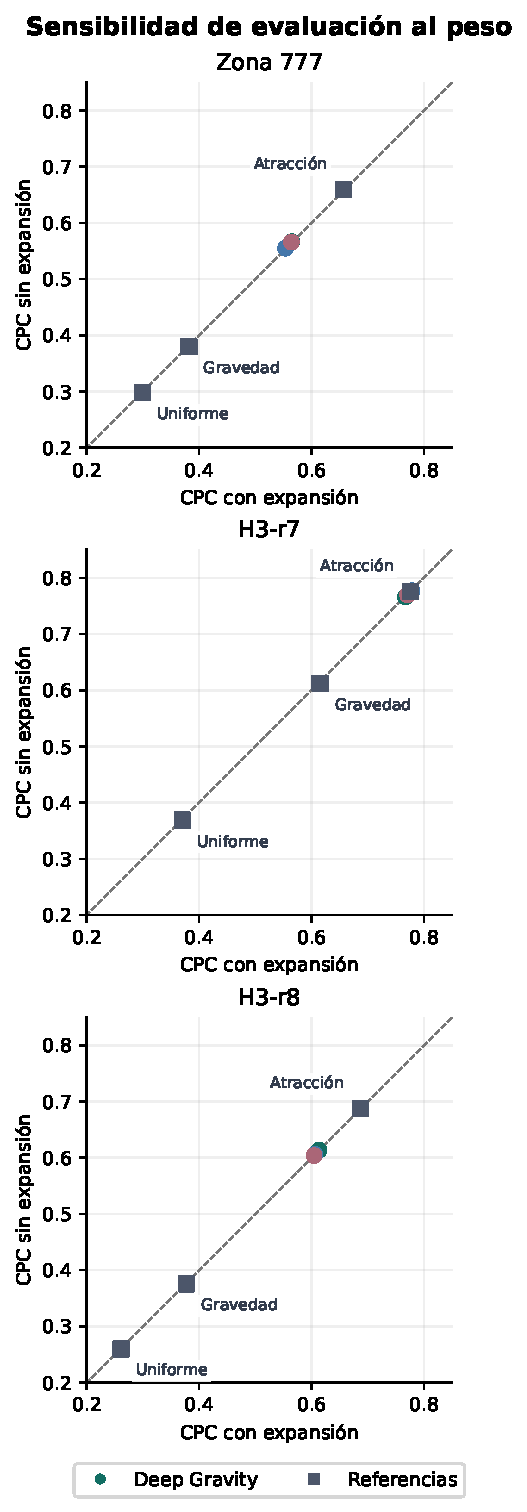
\includegraphics[width=\textwidth]{figures/sensibilidad_pesos.pdf}
\caption{Sensibilidad del CPC de prueba al peso de evaluación. El eje horizontal usa masa expandida y el vertical conteos OD sin expansión; los círculos corresponden a las tres semillas de Deep Gravity y los cuadrados a los modelos de referencia. Cada punto reutiliza probabilidades congeladas y conserva los parámetros de las referencias ajustadas con peso expandido. La diagonal discontinua representa igualdad entre ambas métricas. Fuente: elaboración propia a partir de la evaluación de sensibilidad mensual.}
\label{fig:sensibilidad_pesos}
\end{figure}

El cambio de ponderación no modificó la lectura comparativa principal. Los CPC medios de Deep Gravity fueron 0,5623 en Zona 777, 0,7711 en H3-r7 y 0,6077 en H3-r8 al usar conteos sin expansión, frente a 0,5609, 0,7722 y 0,6079 con masa expandida. La atracción entrenada siguió sobre la media de la red en las tres representaciones. La figura debe leerse como una sensibilidad de evaluación al uso del peso, no como evidencia de que los modelos tendrían el mismo comportamiento después de reentrenarse con otra función de pérdida.

\subsection{Recursos de ejecución}
\label{sec:recursos_ejecucion}

La Tabla~\ref{tab:costos_ejecucion} registra los recursos observados durante las épocas de entrenamiento y validación. Estos tiempos excluyen carga inicial y escritura de \textit{checkpoints}, por lo que el total es una cota inferior del costo operativo y no un presupuesto integral de ejecución.

\begin{table}[htbp]
\centering
\small
\caption{Recursos observados para las nueve corridas mensuales. Las horas corresponden a entrenamiento y validación; la memoria es el máximo registrado en las corridas de cada fila; el tamaño de artefactos se convierte de bytes a GiB ($2^{30}$ bytes) y se redondea a dos decimales. Fuente: elaboración propia a partir del registro de costos e incidencias del experimento mensual.}
\label{tab:costos_ejecucion}
\begin{tabular*}{\textwidth}{@{\extracolsep{\fill}}lrrrr@{}}
\toprule
\textbf{Rama} & \textbf{Corridas} & \textbf{Horas} & \textbf{Memoria máx. (GiB)} & \textbf{Artefactos (GiB)} \\
\midrule
Zona 777 & 3 & 2,62 & 0,53 & 2,33 \\
H3-r7 & 3 & 0,19 & 0,53 & 1,99 \\
H3-r8 & 3 & 6,65 & 0,83 & 2,95 \\
\midrule
Total de nueve corridas & 9 & 9,46 & 0,83 & 7,27 \\
\bottomrule
\end{tabular*}
\end{table}

Las nueve corridas acumularon 9,46 horas de entrenamiento y validación. El desglose fue 0,19 horas en H3-r7, 2,62 horas en Zona 777 y 6,65 horas en H3-r8. El máximo de memoria de proceso observado fue 0,834 GiB. Estas cifras describen los recursos medidos, no el costo operativo completo.

Se registraron dos incidencias sin efecto sobre los resultados de prueba. Antes de la primera época, una corrida de Zona 777 no resolvía un parámetro de hilos de CPU; la corrección se aplicó antes de producir entrenamiento o prueba y no se contabilizó como una inicialización adicional. Más tarde, un primer intento de verificación no pudo serializar una ruta relativa después de crear archivos parciales de reproducción. La verificación final se ejecutó en un directorio nuevo y los archivos parciales quedaron fuera de la evidencia. Ninguna incidencia modificó \textit{checkpoints}, resultados congelados ni la liberación de prueba.

Los desgloses por corrida, origen y \textit{tile}, junto con las verificaciones de conservación de masa y los replays técnicos, permanecen en el respaldo reproducible.

\subsection{Resultado del análisis complementario de atribuciones predictivas}
\label{sec:resultado_xai}

El análisis complementario evaluó tres aproximaciones para atribuir cambios en la log-probabilidad condicional de un destino dentro del soporte completo de cada origen. Las explicaciones se definieron como sensibilidades predictivas dependientes de la salida, de la muestra y de las referencias de entrenamiento. No se interpretaron como efectos causales.

La primera aproximación, basada en gradientes integrados, no acreditó completitud para una consulta crítica aun al aumentar la cuadratura hasta 4.096 nodos. La segunda, basada en permutaciones agrupadas, no acreditó la estabilidad entre dos conjuntos independientes de fondos en dos de las tres inicializaciones de la primera consulta obligatoria. La tercera, basada en valores de Shapley exactos para grupos jerárquicos, acreditó una primera consulta con 24 fondos por conjunto, pero una segunda consulta crítica no alcanzó la estabilidad requerida de los tres supergrupos con 24 ni con 48 fondos.

Ninguna aproximación superó todos los controles definidos antes de la ejecución. Por ello, no se publican rankings, atribuciones, figuras SHAP ni casos locales. El resultado es metodológico: bajo las configuraciones evaluadas no se obtuvieron atribuciones suficientemente estables para una interpretación sustantiva de las características territoriales. Este desenlace limita la interpretabilidad disponible, pero no modifica las métricas predictivas ni las comparaciones con referencias, que se obtuvieron con un protocolo de evaluación distinto.

\subsection{Discusión y amenazas a la validez}
\label{sec:discusion_amenazas_validez}

La evaluación muestra que Deep Gravity puede ejecutarse de forma trazable sobre la cohorte DTPM y producir una distribución de destinos que supera las referencias uniforme y de gravedad exponencial en las tres representaciones examinadas. Sin embargo, la referencia de atracción entrenada obtiene un CPC medio mayor en las tres ramas. Este resultado evita presentar la red como una mejora general sobre todas las referencias y concentra la interpretación en las condiciones concretas de la evaluación.

La reproducción técnica previa del código con datos de Nueva York se conserva como antecedente de compatibilidad de implementación. No reproduce el contexto empírico de Santiago ni funciona como un control equivalente, por lo que sus métricas no se comparan con los CPC de este capítulo.

La discretización espacial modifica el problema evaluado. H3-r7, H3-r8 y Zona 777 no sólo difieren en tamaño o forma de unidad: cambian los destinos disponibles, la densidad de pares OD positivos, la masa de prueba y la agregación de atributos. La sensibilidad observada entre representaciones es informativa para describir ese efecto de agregación, pero no permite declarar una resolución ganadora a partir del CPC global.

La validez temporal queda acotada a las 29 fechas disponibles de noviembre de 2024. La validez espacial queda acotada a una sola partición de origen, concentrada en un \textit{tile} de prueba, y a las 34 comunas del dominio definido. El piloto comparte la geografía de prueba y una de las fechas del agregado mensual. En consecuencia, los resultados no constituyen una validación temporal ni espacial independiente del piloto.

La fuente DTPM representa viajes reconstruibles de transporte público y no toda la movilidad urbana. La distribución predicha está condicionada al flujo saliente observado, por lo que no estima la generación de viajes por origen. Además, la cobertura de OpenStreetMap corresponde a una instantánea anterior a los viajes y la interpolación del Censo 2024 supone distribución uniforme dentro de cada geometría censal. Las decisiones de reconstrucción de viajes, exclusión de zonas sin polígono y asignación a unidades espaciales también condicionan el resultado.

Las tres inicializaciones permiten describir variación de entrenamiento, pero no reemplazan particiones espaciales adicionales ni una muestra poblacional de experimentos. El resultado no validado del análisis de atribuciones añade una limitación específica: los resultados predictivos no pueden acompañarse de una explicación estable de la contribución de cada atributo bajo las configuraciones ensayadas. Una extensión futura debería separar explícitamente la validación temporal y espacial, incorporar particiones adicionales y definir un protocolo explicativo con controles que pueda acreditar estabilidad antes de interpretar atribuciones.


\newpage
\secnumbersection{CONCLUSIONES}
\label{sec:cap6}

Esta memoria evaluó el modelo \textit{Deep Gravity} para la distribución de flujos de movilidad en el transporte público de Santiago de Chile, con el objetivo de estudiar la sensibilidad del desempeño predictivo frente a la discretización espacial. A partir de una cohorte común de 60.511.977 viajes canónicos DTPM, observados entre el 1 y el 29 de noviembre de 2024 en un dominio de 34 comunas, se construyeron tres representaciones espaciales ---Zona~777 (793 unidades), H3-r7 (223 celdas) y H3-r8 (1.210 celdas)--- y se entrenaron nueve modelos mensuales con tres inicializaciones por rama. La evaluación comparó \textit{Deep Gravity} frente a tres referencias ---uniforme, de atracción entrenada y de gravedad exponencial--- mediante el \textit{Common Part of Commuters} (CPC), liberando la prueba una sola vez después de congelar todos los \textit{checkpoints} seleccionados por validación.

Los resultados principales del experimento mensual se resumen a continuación. \textit{Deep Gravity} obtuvo un CPC medio de prueba de 0,5609 en Zona~777, 0,7722 en H3-r7 y 0,6079 en H3-r8, con desviaciones estándar muestrales inferiores a 0,007 entre las tres inicializaciones. La red superó las referencias uniforme y de gravedad exponencial en las tres ramas. Frente a la atracción entrenada, quedó 14,68\% por debajo en Zona~777, 0,46\% por debajo en H3-r7 y 11,48\% por debajo en H3-r8. El casi empate de H3-r7, frente a las brechas de las otras dos ramas, muestra que el desempeño relativo de \textit{Deep Gravity} es sensible a la discretización espacial.

La sensibilidad al peso de evaluación mostró que el cambio de masa expandida a conteos sin expansión no alteró la lectura comparativa. La conservación de masa se verificó con un error máximo absoluto por origen de $1{,}863 \times 10^{-9}$. En cuanto al análisis complementario de explicabilidad, las tres aproximaciones evaluadas ---gradientes integrados, SHAP por permutaciones agrupadas y valores de Shapley exactos para grupos jerárquicos--- no acreditaron todos los controles de completitud y estabilidad predefinidos, por lo que no se publican atribuciones, rankings ni figuras SHAP.

Las tres representaciones comparten la misma cohorte de viajes, pero difieren en el número de destinos por origen, la densidad de pares OD positivos, la masa de prueba y la agregación de los atributos territoriales. La respuesta a la pregunta del título se obtiene comparando la red con sus referencias dentro de cada rama: el cambio de esas brechas relativas demuestra sensibilidad del desempeño a la discretización espacial.


\subsection{Cumplimiento de objetivos}

A continuación se examina el cumplimiento de cada uno de los seis objetivos específicos formulados en la Sección~\ref{sec:objetivos_especificos}.

\textbf{Objetivo~1: Auditar y adaptar el código de referencia.} Se completó una auditoría técnica de la implementación de \textit{scikit-mobility} y se verificó su funcionamiento mediante una corrida de compatibilidad con datos de Nueva York. Esta corrida constituye un antecedente de compatibilidad de implementación, no una demostración de desempeño científico para Santiago. El pipeline resultante registra configuración efectiva, semillas, versiones, hashes de entradas, particiones, métricas y \textit{checkpoints} en un directorio exclusivo por corrida, lo que permite verificar la procedencia de cada resultado.

\textbf{Objetivo~2: Reconstruir viajes canónicos, definir una cohorte común y delimitar el núcleo urbano.} Se reconstruyeron los viajes canónicos mediante la unión de las tablas DTPM de viajes y etapas, exigiendo secuencia completa de etapas, bajada válida en la etapa final y coordenadas dentro de los rangos UTM de control. De los 86.327.914 viajes de la entrega procesable, 25.325.042 (29,34\%) se excluyeron porque no registraban bajada en la etapa final. El dominio de estudio se delimitó a 34 comunas, con exclusión posterior de las zonas 848, 849 y 852 por carecer de polígono oficial verificable. La cascada completa de la Tabla~\ref{tab:cascada_filtros_dtpm} conduce a una cohorte comparativa de 60.511.977 viajes con 85.774.522,4070 de masa expandida, compartida por las tres ramas.

\textbf{Objetivo~3: Construir representaciones comparables y seleccionar candidatas.} La Tabla~\ref{tab:factibilidad_h3} documenta la evaluación de H3-r3 a H3-r8 con conservación de cohorte y masa, un mínimo de 100 orígenes activos y un límite de 128 MiB para la matriz densa de puntajes de una pasada. H3-r3 a H3-r6 aportaron entre 1 y 44 orígenes activos y se descartaron por soporte demasiado grueso; H3-r7 y H3-r8 aportaron 220 y 1.194, respectivamente, por lo que pasaron al piloto junto con Zona~777 y se mantuvieron en el experimento mensual. Las tres representaciones finales usan adaptadores espaciales explícitos sobre la misma cohorte fuente.

\textbf{Objetivo~4: Construir atributos con fuentes, unidades y procedimientos explícitos.} Se construyó un vector de 19 atributos por ubicación: una densidad de población censal (Censo 2024, interpolada por fracción de área), cinco coberturas de uso de suelo, tres densidades de longitud vial y diez variables de servicios. Cada par OD se representa con los 19 atributos del origen, los 19 del destino y la distancia geodésica, sumando 39 entradas. La normalización se estimó exclusivamente con orígenes activos de entrenamiento de cada rama y escenario, impidiendo que el conjunto de prueba interviniera en la estandarización.

\textbf{Objetivo~5: Entrenar y evaluar \textit{Deep Gravity} frente a tres referencias.} Se ejecutaron nueve corridas mensuales con tres representaciones y tres inicializaciones, utilizando el soporte completo de destinos. \textit{Deep Gravity} superó la referencia uniforme y la de gravedad exponencial en las tres ramas, con diferencias relativas de CPC de 87--133\% y de 25--61\%, respectivamente. Frente a la atracción entrenada, las diferencias fueron $-14{,}68\%$ en Zona~777, $-0{,}46\%$ en H3-r7 y $-11{,}48\%$ en H3-r8. Todas estas comparaciones se calcularon dentro de cada rama y muestran que la discretización modifica el margen relativo de la red. Bajo la configuración evaluada, el experimento no permite atribuir esta diferencia a un mecanismo concreto ni evaluar la transferencia del modelo a ciudades sin flujos de entrenamiento.

\textbf{Objetivo~6: Evaluar la viabilidad de obtener atribuciones predictivas estables.} Se implementaron y evaluaron tres aproximaciones de XAI con controles predefinidos de completitud, convergencia y estabilidad. Los gradientes integrados no acreditaron completitud para una consulta crítica. El método por permutaciones no acreditó estabilidad entre fondos independientes en dos de tres inicializaciones. El método exacto jerárquico acreditó una primera consulta, pero no una segunda consulta crítica. La evaluación de viabilidad se completó, pero no se obtuvieron atribuciones suficientemente estables para una interpretación sustantiva. El resultado delimita el alcance del análisis complementario y justifica no publicar atribuciones, rankings ni figuras XAI.


\subsection{Contribuciones}

Las contribuciones de esta memoria se enumeran a continuación.

\begin{enumerate}
    \item \textbf{Evaluación reproducible de \textit{Deep Gravity} para transporte público observable en Santiago.} El trabajo adapta y evalúa el modelo con viajes reconstruibles desde DTPM y atributos territoriales de Censo 2024 y OpenStreetMap. La evaluación se realizó sobre tres representaciones espaciales y con un protocolo de prueba congelado.

    \item \textbf{Metodología de comparación entre discretizaciones con cohorte común.} El diseño experimental separa el núcleo común de viajes de los adaptadores espaciales, permitiendo describir la sensibilidad del desempeño a la discretización sin confundir cambios de datos con cambios de representación. Su adaptación a otras ciudades o modelos requiere una verificación independiente de sus supuestos y resultados.

    \item \textbf{Pipeline con trazabilidad integral.} Cada corrida conserva semillas, hashes de entradas, versiones de código, particiones deterministas, métricas por origen y \textit{checkpoints} en un directorio exclusivo. La prueba se libera una sola vez después de congelar las decisiones de validación, sin selección post-hoc de semillas ni de representaciones. La conservación de masa se verifica explícitamente.

    \item \textbf{Resultado metodológico sobre los límites de XAI.} La evaluación sistemática de tres aproximaciones de explicabilidad, con controles predefinidos de completitud y estabilidad, documenta que ninguna acreditó todos los controles en las configuraciones evaluadas. Esto refuerza la necesidad de verificar dichos controles antes de interpretar o publicar atribuciones.

    \item \textbf{Caracterización de la referencia de atracción.} Entre las referencias evaluadas, la atracción entrenada alcanzó el mayor CPC medio en las tres representaciones. Este resultado define un punto de comparación para estudios posteriores, sin identificar por sí mismo el mecanismo que explica la diferencia.
\end{enumerate}


\subsection{Limitaciones}

Las limitaciones de este trabajo se agrupan en tres categorías.

\textbf{Limitaciones de datos.} La fuente de movilidad se restringe a los viajes reconstruibles desde DTPM durante las 29 fechas disponibles de noviembre de 2024. No cubre viajes en modos no observables (caminata pura, taxi, vehículo particular, bicicleta), por lo que los resultados no representan la totalidad de la movilidad urbana. El modelo requiere como entrada el flujo saliente observado por origen ($O_i$), lo cual limita su autonomía respecto a datos de validación. El diagnóstico de la Sección~\ref{sec:cobertura_atributos_osm} cuantificó la presencia de los atributos OSM por unidad y encontró menores medianas hacia el cuartil periférico en las tres representaciones; no estimó la completitud externa de OSM ni su asociación con el nivel socioeconómico. Una ausencia cartografiada tampoco demuestra una ausencia real de servicios. La instantánea OSM utilizada (2024-01-01) antecede a los viajes, y la interpolación areal del Censo 2024 supone distribución uniforme dentro de cada geometría censal.

\textbf{Limitaciones del diseño experimental.} Las tres inicializaciones caracterizan la variación de entrenamiento bajo una sola partición espacial fija (un \textit{tile} de prueba), por lo que no estiman incertidumbre poblacional ni variación entre particiones. No se dispone de una validación temporal independiente: el experimento mensual contiene el día del piloto y comparte su geografía de prueba. No se comparó \textit{Deep Gravity} contra modelos de oportunidades intervinientes (PWO, modelo unificado de Liu y Yan) ni contra arquitecturas de grafos (GNN), que el trabajo relacionado identifica como alternativas relevantes. El \textit{dropout} efectivo fue cero y no se exploró la sensibilidad a hiperparámetros de la arquitectura, como profundidad, ancho de capas o función de optimización.

\textbf{Limitaciones de alcance.} La evaluación distribuye flujos condicionados al flujo saliente observado; no predice la generación total de viajes por origen ni fechas futuras. Las conclusiones se limitan al transporte público observable en DTPM dentro de las 34 comunas del dominio de estudio. No se integró la generación de flujos con un proceso de planificación de transporte ni de optimización de rutas o frecuencias.


\subsection{Trabajo futuro}

La prioridad es repetir la evaluación con particiones espaciales y períodos temporales independientes, definiendo antes de la prueba las reglas de agregación y los criterios de estabilidad. Esto permitiría examinar cuánto dependen los resultados de la partición fija y del período disponible en esta memoria.

También se puede ampliar la comparación con modelos de oportunidades, variantes de arquitectura e información territorial complementaria. Tales extensiones deben tratarse como hipótesis de diseño: el experimento actual no permite anticipar qué cambio reduciría la diferencia con la referencia de atracción.

Por último, una evaluación de transferencia hacia contextos sin flujos de entrenamiento exigiría modelar o medir el flujo saliente $O_i$ y validarlo de forma independiente. En XAI, futuras configuraciones podrían contrastar arquitecturas, regularización y conjuntos de referencia bajo los mismos controles de completitud y estabilidad; el diseño realizado no permite identificar cuál de esos cambios resolvería las limitaciones observadas.


\subsection{Reflexión final}

Esta memoria demuestra que \textit{Deep Gravity} puede ejecutarse de forma trazable y reproducible sobre datos reales de transporte público en Santiago de Chile, y que sus distribuciones de destino superan las referencias uniforme y gravitacional en las tres discretizaciones evaluadas. Bajo el protocolo aplicado, la referencia de atracción entrenada obtuvo el mayor CPC medio. Una evaluación de transferencia hacia contextos sin flujos de entrenamiento requeriría un diseño distinto, que incorpore una estrategia para estimar el flujo saliente y una validación independiente.

La comparación con referencias dentro de cada rama responde la pregunta central de esta memoria: el desempeño relativo de \textit{Deep Gravity} es sensible a la discretización espacial. La red casi igualó a la atracción en H3-r7, mientras que quedó 14,68\% por debajo en Zona~777 y 11,48\% por debajo en H3-r8. La representación del espacio condiciona, por tanto, el margen predictivo observado, además de los atributos construidos y el soporte de la tarea.

El análisis complementario de explicabilidad no obtuvo atribuciones que superaran todos los controles predefinidos. Por ello, las atribuciones no se interpretan ni se publican; los controles de completitud y estabilidad deben anteceder cualquier lectura sustantiva de estos resultados.

La trazabilidad del pipeline, desde la reconstrucción de la cohorte hasta la liberación de la prueba, aporta las condiciones necesarias para inspeccionar, reproducir o contrastar estos resultados con otras particiones, períodos y configuraciones.


\newpage
\phantomsection
\addcontentsline{toc}{section}{ANEXOS}

\newcounter{anexo}
\renewcommand{\theanexo}{\Alph{anexo}}
\newcommand{\anexotitulo}[2]{%
  \refstepcounter{anexo}%
  \setcounter{table}{0}%
  \renewcommand{\thetable}{\theanexo.\arabic{table}}%
  \subsection*{Anexo~\theanexo. #1}%
  \phantomsection
  \addcontentsline{toc}{subsection}{Anexo~\theanexo. #1}%
  \label{#2}%
}

\anexotitulo{Diccionario de atributos territoriales}{anexo:diccionario_atributos}

Este anexo documenta los 19 atributos de localización que integran el vector de entrada aprobado para el modelo. Las variables diagnósticas se reportan por separado y el flujo observado constituye la variable objetivo. Las transformaciones se ajustan únicamente con los orígenes activos del conjunto de entrenamiento de cada rama y escenario.

\begin{table}[H]
  \centering
  \scriptsize
  \caption{Atributos de población, uso de suelo y red vial del vector de entrada.}
  \label{tab:anexo_atributos_base}
  \begin{tabularx}{\textwidth}{@{}p{0.34\textwidth}p{0.42\textwidth}X@{}}
    \toprule
    \textbf{Atributo} & \textbf{Fuente y construcción} & \textbf{Unidad y transformación} \\
    \midrule
    \texttt{population\_census\_2024\_per\_km2} &
    Censo 2024 del INE; asignación areal de población y división por el área métrica de la unidad. &
    personas/km$^2$; $\log(1+x)$ y estandarización $z$. \\
    \texttt{landuse\_residential\_share} &
    OpenStreetMap (corte 2024-01-01); unión de polígonos residenciales recortados y división por el área de la unidad. &
    km$^2$/km$^2$; estandarización $z$. \\
    \texttt{landuse\_commercial\_share} &
    OpenStreetMap (corte 2024-01-01); unión de polígonos comerciales recortados y división por el área de la unidad. &
    km$^2$/km$^2$; estandarización $z$. \\
    \texttt{landuse\_industrial\_share} &
    OpenStreetMap (corte 2024-01-01); unión de polígonos industriales recortados y división por el área de la unidad. &
    km$^2$/km$^2$; estandarización $z$. \\
    \texttt{landuse\_retail\_share} &
    OpenStreetMap (corte 2024-01-01); unión de polígonos de comercio minorista recortados y división por el área de la unidad. &
    km$^2$/km$^2$; estandarización $z$. \\
    \texttt{landuse\_natural\_share} &
    OpenStreetMap (corte 2024-01-01); unión de polígonos naturales recortados y división por el área de la unidad. &
    km$^2$/km$^2$; estandarización $z$. \\
    \texttt{road\_residential\_km\_per\_km2} &
    OpenStreetMap; unión de líneas residenciales recortadas y división por el área de la unidad. &
    km/km$^2$; $\log(1+x)$ y estandarización $z$. \\
    \texttt{road\_main\_km\_per\_km2} &
    OpenStreetMap; unión de líneas principales recortadas y división por el área de la unidad. &
    km/km$^2$; $\log(1+x)$ y estandarización $z$. \\
    \texttt{road\_other\_km\_per\_km2} &
    OpenStreetMap; unión de las demás líneas viales recortadas y división por el área de la unidad. &
    km/km$^2$; $\log(1+x)$ y estandarización $z$. \\
    \bottomrule
  \end{tabularx}
\end{table}

\begin{table}[H]
  \centering
  \scriptsize
  \caption{Atributos de puntos de interés y superficie por familia temática.}
  \label{tab:anexo_atributos_poi}
  \begin{tabularx}{\textwidth}{@{}p{0.31\textwidth}p{0.43\textwidth}X@{}}
    \toprule
    \textbf{Atributo} & \textbf{Fuente y construcción} & \textbf{Unidad y transformación} \\
    \midrule
    \texttt{transport\_poi\_per\_km2} &
    OpenStreetMap; nodos estrictamente interiores, deduplicados por homónimos nodo--área, categoría y coincidencia espacial, divididos por el área de la unidad. &
    objetos/km$^2$; $\log(1+x)$ y estandarización $z$. \\
    \texttt{transport\_area\_share} &
    OpenStreetMap; unión de las superficies de transporte recortadas y división por el área de la unidad. &
    km$^2$/km$^2$; estandarización $z$. \\
    \texttt{food\_poi\_per\_km2} &
    OpenStreetMap; nodos estrictamente interiores, deduplicados por homónimos nodo--área, categoría y coincidencia espacial, divididos por el área de la unidad. &
    objetos/km$^2$; $\log(1+x)$ y estandarización $z$. \\
    \texttt{food\_area\_share} &
    OpenStreetMap; unión de las superficies de alimentación recortadas y división por el área de la unidad. &
    km$^2$/km$^2$; estandarización $z$. \\
    \texttt{health\_poi\_per\_km2} &
    OpenStreetMap; nodos estrictamente interiores, deduplicados por homónimos nodo--área, categoría y coincidencia espacial, divididos por el área de la unidad. &
    objetos/km$^2$; $\log(1+x)$ y estandarización $z$. \\
    \texttt{health\_area\_share} &
    OpenStreetMap; unión de las superficies de salud recortadas y división por el área de la unidad. &
    km$^2$/km$^2$; estandarización $z$. \\
    \texttt{education\_poi\_per\_km2} &
    OpenStreetMap; nodos estrictamente interiores, deduplicados por homónimos nodo--área, categoría y coincidencia espacial, divididos por el área de la unidad. &
    objetos/km$^2$; $\log(1+x)$ y estandarización $z$. \\
    \texttt{education\_area\_share} &
    OpenStreetMap; unión de las superficies educacionales recortadas y división por el área de la unidad. &
    km$^2$/km$^2$; estandarización $z$. \\
    \texttt{retail\_poi\_per\_km2} &
    OpenStreetMap; nodos estrictamente interiores, deduplicados por homónimos nodo--área, categoría y coincidencia espacial, divididos por el área de la unidad. &
    objetos/km$^2$; $\log(1+x)$ y estandarización $z$. \\
    \texttt{retail\_area\_share} &
    OpenStreetMap; unión de las superficies de comercio minorista recortadas y división por el área de la unidad. &
    km$^2$/km$^2$; estandarización $z$. \\
    \bottomrule
  \end{tabularx}
\end{table}

La distancia $d_{ij}$ se calcula como distancia geodésica esférica WGS84 entre los centroides representativos de los pares origen--destino y se incorpora al vector como medida de separación espacial. Una ruta por la red requiere información adicional de infraestructura y operación. Las capas territoriales pueden superponerse, por lo que sus proporciones se analizan por familia. Para OpenStreetMap, un valor cero registra ausencia de objetos mapeados conforme a la regla aplicada.

\clearpage
\anexotitulo{Trazabilidad de las corridas mensuales}{anexo:corridas_mensuales}

Este anexo individualiza las nueve corridas del experimento mensual: tres inicializaciones independientes en cada representación. La época seleccionada corresponde al mayor CPC global de validación de la trayectoria, conservando la primera época ante empate; la época final indica cuándo se detuvo la corrida. Las dos continuaciones autorizadas partieron del límite inicial de 200 épocas y conservaron datos, particiones, atributos, arquitectura, optimizador y regla de selección. Todas las corridas cerraron por meseta de validación.

\begin{table}[H]
  \centering
  \scriptsize
  \caption{Corridas del experimento mensual y selección por validación.}
  \label{tab:anexo_corridas}
  \resizebox{\textwidth}{!}{%
    \begin{tabular}{@{}lrrrrll@{}}
      \toprule
      \textbf{Representación} & \textbf{Semilla} & \textbf{Época seleccionada} & \textbf{Época final} & \textbf{CPC validación} & \textbf{Extensión} & \textbf{Cierre} \\
      \midrule
      Zona 777 & 20260909 & 196 & 226 & 0,532453 & 200--226 & Meseta \\
      Zona 777 & 20260910 & 94  & 124 & 0,525924 & ---      & Meseta \\
      Zona 777 & 20260911 & 74  & 104 & 0,517290 & ---      & Meseta \\
      H3-r7    & 20260909 & 72  & 97  & 0,737286 & ---      & Meseta \\
      H3-r7    & 20260910 & 162 & 192 & 0,734555 & ---      & Meseta \\
      H3-r7    & 20260911 & 69  & 99  & 0,732907 & ---      & Meseta \\
      H3-r8    & 20260909 & 158 & 188 & 0,600163 & ---      & Meseta \\
      H3-r8    & 20260910 & 188 & 218 & 0,594110 & 200--218 & Meseta \\
      H3-r8    & 20260911 & 137 & 167 & 0,589980 & ---      & Meseta \\
      \bottomrule
    \end{tabular}%
  }
\end{table}

La prueba se evaluó después de fijar y congelar los \textit{checkpoints} seleccionados por validación. Los resultados de las tres semillas se presentan completos en el Capítulo 5; esta tabla conserva la trazabilidad de la selección.

\clearpage
\anexotitulo{Controles de soporte, conservación de masa y ejecución}{anexo:controles_ejecucion}

Este anexo reúne los controles de reproducibilidad y el detalle de los recursos medidos junto con los denominadores de la repetición independiente, la conservación del flujo por origen, el detalle por corrida y las incidencias técnicas resueltas.

\subsubsection*{Soporte de prueba, repetición independiente y conservación de masa}

\begin{table}[H]
  \centering
  \scriptsize
  \caption{Controles de soporte, repetición independiente y conservación de masa.}
  \label{tab:anexo_controles_soporte}
  \resizebox{\textwidth}{!}{%
    \begin{tabular}{@{}lrrrrrr@{}}
      \toprule
      \textbf{Representación} & \textbf{Orígenes/destinos prueba} & \textbf{Unidades sin origen} & \textbf{CPC congelado} & \textbf{CPC repetido} & \textbf{Diferencia CPC} & \textbf{Máx. error por origen} \\
      \midrule
      Zona 777 & 101/793  & 0  & 0,5647245226 & 0,5647245225 & $9{,}576\times10^{-11}$ & $9{,}313\times10^{-10}$ \\
      H3-r7    & 32/223   & 5  & 0,7670518160 & 0,7670518160 & $3{,}483\times10^{-11}$ & $1{,}863\times10^{-9}$ \\
      H3-r8    & 189/1210 & 21 & 0,6132965073 & 0,6132965073 & $9{,}350\times10^{-12}$ & $1{,}630\times10^{-9}$ \\
      \bottomrule
    \end{tabular}%
  }
\end{table}

\noindent\footnotesize\textit{Nota.} El error máximo corresponde al máximo entre las tres semillas y los dos esquemas de ponderación. La repetición independiente usa la semilla 20260909 y el conjunto completo de destinos. El soporte de prueba comprende los orígenes asignados al bloque de prueba; las unidades sin origen se registran por separado y se excluyen del cálculo del CPC.\normalsize

La repetición independiente recuperó el CPC congelado de cada representación, con diferencias inferiores a $10^{-6}$. Las nueve corridas preservaron el flujo por origen; el mayor error observado fue $1{,}863\times10^{-9}$. Estos controles verifican la consistencia técnica de la ejecución; la evaluación espacial y temporal se desarrolla mediante el protocolo del Capítulo 5.

\subsubsection*{Recursos medidos por corrida}

\begin{table}[H]
  \centering
  \small
  \caption{Tiempo de entrenamiento, memoria RAM y tamaño de artefactos por corrida.}
  \label{tab:anexo_recursos}
  \begin{tabular}{@{}lrrrr@{}}
    \toprule
    \textbf{Representación} & \textbf{Semilla} & \textbf{Entrenamiento (h)} & \textbf{RAM máx. (GiB)} & \textbf{Artefactos (GiB)} \\
    \midrule
    Zona 777 & 20260909 & 1,30 & 0,53 & 1,16 \\
    Zona 777 & 20260910 & 0,72 & 0,53 & 0,64 \\
    Zona 777 & 20260911 & 0,60 & 0,53 & 0,53 \\
    H3-r7    & 20260909 & 0,05 & 0,53 & 0,50 \\
    H3-r7    & 20260910 & 0,10 & 0,53 & 0,99 \\
    H3-r7    & 20260911 & 0,05 & 0,53 & 0,51 \\
    H3-r8    & 20260909 & 2,19 & 0,78 & 0,97 \\
    H3-r8    & 20260910 & 2,50 & 0,83 & 1,12 \\
    H3-r8    & 20260911 & 1,95 & 0,78 & 0,86 \\
    \midrule
    Suma/máximo (9 corridas) & --- & 9,46 & 0,83 & 7,27 \\
    \bottomrule
  \end{tabular}
\end{table}

Las horas corresponden a las épocas de entrenamiento y validación. La carga inicial y la escritura de \textit{checkpoints} se registran fuera de esa medida, por lo que las horas son una cota inferior del tiempo total de ejecución. La RAM se informa como máximo observado y el tamaño corresponde a los artefactos conservados de cada corrida. Las condiciones de ejecución difieren entre ramas, por lo que la tabla reporta tiempo de entrenamiento y validación en vez de tiempo calendario.

\subsubsection*{Incidencias técnicas resueltas}

\begin{table}[H]
  \centering
  \small
  \caption{Incidencias técnicas y efecto sobre los resultados reportados.}
  \label{tab:anexo_incidencias}
  \begin{tabularx}{\textwidth}{@{}p{0.24\textwidth}p{0.48\textwidth}X@{}}
    \toprule
    \textbf{Alcance} & \textbf{Incidencia y resolución} & \textbf{Efecto} \\
    \midrule
    Zona 777, semilla 20260909 &
    Se detectó la ausencia del parámetro de hilos de CPU antes de iniciar el entrenamiento. Se corrigió antes de entrenar y evaluar la corrida. &
    La corrección se realizó antes del entrenamiento y la evaluación; la corrida conservó su plan y sus resultados. \\
    Cierre y repetición independiente &
    Una ruta relativa de serialización se detectó luego de generar productos parciales. La repetición se ejecutó en un directorio nuevo y se excluyeron los productos parciales. &
    Los \textit{checkpoints} congelados y la evaluación de prueba conservaron los resultados reportados. \\
    \bottomrule
  \end{tabularx}
\end{table}


\newpage
% Bibliografía estilo APA:
\bibliographystyle{apalike-es}
\bibliography{bibliografia}{}

\end{document}
